\documentclass[aspectratio=169,11pt]{beamer}

\usetheme{Madrid}
\usecolortheme{default}
\setbeamertemplate{navigation symbols}{}
\setbeamertemplate{footline}[frame number]

\usepackage[utf8]{inputenc}
\usepackage[T1]{fontenc}
\usepackage[brazil]{babel}
\usepackage{lmodern}
\usepackage{amsmath,amssymb,bm,mathtools}
\usepackage{physics}
\usepackage{tikz}
\usepackage{graphicx}
\usepackage{booktabs}
\usepackage{ragged2e}
\usepackage[most]{tcolorbox}

\definecolor{myblue}{RGB}{0,86,125}
\definecolor{mycyan}{RGB}{0,183,235}
\definecolor{myred}{RGB}{160,30,30}
\definecolor{mygray}{RGB}{245,247,250}
\definecolor{mydark}{RGB}{40,40,40}

\setbeamercolor{structure}{fg=myblue}
\setbeamercolor{frametitle}{fg=white,bg=myblue}
\setbeamercolor{title}{fg=white}
\setbeamercolor{block title}{fg=white,bg=myblue}
\setbeamercolor{block body}{bg=mygray,fg=black}
\setbeamercolor{alerted text}{fg=myred}

\newtcolorbox{mybox}[1][]{
  enhanced,
  colback=mygray,
  colframe=myblue,
  boxrule=0.8pt,
  arc=2mm,
  left=2mm,right=2mm,top=1.5mm,bottom=1.5mm,
  #1
}

\newtcolorbox{eqbox}[1][]{
  enhanced,
  colback=white,
  colframe=mycyan,
  boxrule=0.8pt,
  arc=2mm,
  left=1.5mm,right=1.5mm,top=1mm,bottom=1mm,
  #1
}



\newcommand{\notas}[1]{%
\begin{tikzpicture}[remember picture,overlay]
\node[anchor=south west,
      xshift=3mm,
      yshift=3mm,
      draw,
      rectangle,
      rounded corners=2pt,
      fill=white,
      font=\tiny,
      inner sep=2pt]
at (current page.south west)
{Notas: #1};
\end{tikzpicture}
}

\newcommand{\E}{\mathbf{E}}
\newcommand{\D}{\mathbf{D}}
\newcommand{\F}{\mathbf{F}}
\newcommand{\N}{\mathbf{N}}
\newcommand{\rr}{\mathbf{r}}
\newcommand{\rrp}{\mathbf{r}'}
\newcommand{\zhat}{\hat{\mathbf{z}}}

\title{Capítulo 3 -- Eletrostática}
\author{Prof. Dr. Rafael C. R. de Lima}
\institute{UDESC -- CCT}
\date{}

\begin{document}

%------------------------------------------------
\begin{frame}[plain]
    \begin{tikzpicture}[remember picture,overlay]
        \fill[myblue] (current page.south west) rectangle (current page.north east);
        \fill[mycyan,opacity=0.15] ([xshift=-1cm,yshift=1cm]current page.south east) circle (3.2cm);
        \fill[white,opacity=0.08] ([xshift=1cm,yshift=-1cm]current page.north west) circle (2.8cm);
    \end{tikzpicture}
    \vspace{1.0cm}
    {
    \centering
    {
      \usebeamerfont{title}\fontsize{24}{28}\selectfont\bfseries\color{white}
      Capítulo 3 -- Eletrostática\par}
    \vspace{0.45cm}
    {
      \Large\color{white!92}Campo elétrico, lei de Coulomb e potencial escalar\par}
    \vspace{0.8cm}
    {
      \large\color{white!85}Prof. Dr. Rafael C. R. de Lima \;--\; UDESC -- CCT\par}
    \vspace{0.6cm}
    {
      \normalsize\itshape\color{white!80}
      ``O assunto que vou recomendar à sua atenção quase me apavora.\\
      A variedade que apresenta é imensa... O assunto que quero dizer é a eletricidade.''\\
      \vspace{1mm}
      Leonhard Euler (1761)\par}
    }
\end{frame}

%------------------------------------------------
\begin{frame}{Roteiro do capítulo}
\begin{mybox}
\begin{enumerate}
    \item \textbf{3.1 Introdução}: equações diferenciais da eletrostática e significado físico de \(\E(\rr)\).
    \item \textbf{3.1.1 Escopo da eletrostática}: problemas de somação e de contorno.
    \item \textbf{3.2 Lei de Coulomb}: obtenção da forma integral do campo.
    \item \textbf{Exemplo 3.1}: anel, disco e folha infinita uniformemente carregados.
    \item \textbf{3.3 Potencial escalar}: definição, casos particulares e equação de Poisson.
    \item \textbf{Exemplo 3.2}: mudança de escala em distribuições de carga.
    \item \textbf{3.3.1 Força de Coulomb conservativa}: trabalho e independência do caminho.
\end{enumerate}
\end{mybox}
\end{frame}

%------------------------------------------------
\begin{frame}{3.1 Introdução}
\begin{mybox}
\justifying
Na eletrostática, consideramos distribuições de carga \(\rho(\rr)\) independentes do tempo. 
Essas distribuições geram um campo elétrico \(\E(\rr)\) que deve obedecer às equações de Maxwell no regime estático.
\end{mybox}

\vspace{0.2cm}

\begin{columns}[T,onlytextwidth]
\column{0.48\textwidth}
\begin{eqbox}
\begin{equation}
\nabla\times \E(\rr)=0
\label{eq:3.1}
\end{equation}
\end{eqbox}

\column{0.48\textwidth}
\begin{eqbox}
\begin{equation}
 \nabla\cdot \E(\rr)=\rho(\rr)/\epsilon_0
\label{eq:3.2}
\end{equation}
\end{eqbox}
\end{columns}

\vspace{0.2cm}

\begin{block}{Interpretação}
\begin{itemize}
    \item A equação \eqref{eq:3.1} diz que o campo eletrostático é \alert{irrotacional}.
    \item A equação \eqref{eq:3.2} diz que a \alert{fonte} do campo é a densidade de carga.
    \item Conhecendo \(\rho(\rr)\), queremos determinar \(\E(\rr)\) em todo o espaço.
\end{itemize}
\end{block}
\end{frame}

%------------------------------------------------
\begin{frame}{Força, torque e energia}
\begin{mybox}
\justifying
O campo elétrico é relevante porque determina a força e o torque exercidos por uma distribuição \(\rho(\rr)\) sobre uma segunda distribuição \(\rho^\ast(\rr)\).
\end{mybox}

\vspace{0.25cm}

\begin{columns}[T,onlytextwidth]
\column{0.48\textwidth}
\begin{eqbox}
\begin{equation}
\F=\int d^3r\;\rho^\ast(\rr)\,\E(\rr)
\label{eq:3.3}
\end{equation}
\end{eqbox}

\column{0.48\textwidth}
\begin{eqbox}
\begin{equation}
\N=\int d^3r\;\rr\times \rho^\ast(\rr)\E(\rr)
\label{eq:3.4}
\end{equation}
\end{eqbox}
\end{columns}

\vspace{0.25cm}

\begin{block}{Comentário físico}
\justifying
Mesmo quando força e torque não são o foco principal, a \alert{energia eletrostática} associada a \(\E(\rr)\), \(\rho(\rr)\) e \(\rho^\ast(\rr)\) quase sempre é de interesse. 
Por isso, desenvolver expressões equivalentes para o campo e para o potencial será central ao longo do capítulo.
\end{block}
\end{frame}

%------------------------------------------------
\begin{frame}{3.1.1 O escopo da eletrostática}
\begin{columns}[T,onlytextwidth]
\column{0.49\textwidth}
\begin{block}{Problemas de somação}
\justifying
A distribuição \(\rho(\rr)\) é dada \textbf{em todo o espaço}, de uma vez por todas.
Então, determinar \(\E(\rr)\) se reduz, em essência, a calcular integrais sobre as fontes.
\end{block}

\column{0.49\textwidth}
\begin{block}{Problemas de contorno}
\justifying
A função \(\rho(\rr)\) não é totalmente conhecida de antemão. 
A presença de matéria, especialmente condutores e meios polarizáveis, faz a carga se redistribuir e impõe condições adicionais nas interfaces.
\end{block}
\end{columns}

\vspace{0.25cm}

\begin{mybox}
\justifying
Historicamente, essa redistribuição recebe nomes diferentes conforme o material:
\begin{itemize}
    \item \textbf{indução eletrostática} em condutores;
    \item \textbf{polarização elétrica} em não condutores.
\end{itemize}
Neste capítulo, o foco principal está nos \alert{problemas de somação}, enquanto problemas de contorno aparecem mais adiante.
\end{mybox}
\end{frame}

%------------------------------------------------
\begin{frame}{3.2 Lei de Coulomb: ponto de partida}
\begin{mybox}
\justifying
As equações \eqref{eq:3.1} e \eqref{eq:3.2} especificam exatamente o rotacional e a divergência de \(\E(\rr)\). 
Pelo teorema de Helmholtz, isso é suficiente para reconstruir o campo.
\end{mybox}

\vspace{0.25cm}

\begin{eqbox}
\begin{equation}
\E(\rr)=
-\nabla \int d^3r'\,\frac{\nabla'\cdot \E(\rr')}{4\pi\abs{\rr-\rr'}}
+
\nabla\times \int d^3r'\,\frac{\nabla'\times \E(\rr')}{4\pi\abs{\rr-\rr'}}
\label{eq:3.5}
\end{equation}
\end{eqbox}

\vspace{0.2cm}

\begin{block}{Ideia essencial}
\justifying
Como o campo eletrostático satisfaz \(\nabla'\times\E(\rr')=0\), o segundo termo desaparece.
Já a divergência pode ser substituída por \(\rho(\rr')/\epsilon_0\), levando diretamente a uma expressão puramente em termos das fontes.
\end{block}
\end{frame}

%------------------------------------------------
\begin{frame}{Da forma geral à forma eletrostática}
\begin{eqbox}
\begin{equation}
\E(\rr)=
-\nabla \frac{1}{4\pi\epsilon_0}\int d^3r'\,\frac{\rho(\rr')}{\abs{\rr-\rr'}}
\label{eq:3.6}
\end{equation}
\end{eqbox}


\begin{mybox}
\justifying
A derivada pode ser levada para dentro da integral porque o operador \(\nabla\) atua sobre a coordenada de observação \(\rr\), e não sobre a variável de integração \(\rr'\).
\end{mybox}


\begin{eqbox}
\begin{equation}
\nabla\!\left(\frac{1}{\abs{\rr-\rr'}}\right)
=
-\frac{\rr-\rr'}{\abs{\rr-\rr'}^3}
\label{eq:3.7}
\end{equation}
\end{eqbox}


\begin{block}{Consequência}
Substituindo \eqref{eq:3.7} em \eqref{eq:3.6}, obtemos a forma explícita do campo elétrico como superposição das contribuições produzidas por cada elemento de carga.
\end{block}
\end{frame}

%------------------------------------------------
\begin{frame}{Lei de Coulomb em forma integral}
\begin{eqbox}
\begin{equation}
\E(\rr)=
\frac{1}{4\pi\epsilon_0}
\int d^3r'\,\rho(\rr')
\frac{\rr-\rr'}{\abs{\rr-\rr'}^3}
\label{eq:3.8}
\end{equation}
\end{eqbox}

\vspace{0.1cm}

\begin{mybox}
\justifying
A equação \eqref{eq:3.8} mostra que o campo é a soma vetorial de todas as contribuições elementares
\[
d\E=
\frac{1}{4\pi\epsilon_0}\,
\frac{dq\,(\rr-\rr')}{\abs{\rr-\rr'}^3}.
\]
Cada elemento de carga contribui ao longo da reta que liga a fonte ao ponto de observação.
\end{mybox}

\vspace{0.1cm}

\begin{alertblock}{Leitura física}
\justifying
A intensidade decai como \(1/R^2\), enquanto a direção é dada pelo versor radial que aponta da fonte para o ponto onde o campo está sendo calculado.
\end{alertblock}
\end{frame}

%------------------------------------------------
\begin{frame}{Força de Coulomb entre distribuições}
\begin{eqbox}
\begin{equation}
\F=
\frac{1}{4\pi\epsilon_0}
\int d^3r \int d^3r'\,
\rho^\ast(\rr)\rho(\rr')
\frac{\rr-\rr'}{\abs{\rr-\rr'}^3}
\label{eq:3.9}
\end{equation}
\end{eqbox}

\vspace{0.25cm}

\begin{block}{Consequência imediata}
\justifying
Trocando \(\rho\leftrightarrow \rho^\ast\), o integrando muda de sinal, o que implica
\[
\F^\ast=-\F.
\]
Logo, a força entre duas distribuições de carga obedece a uma forma contínua da terceira lei de Newton.
\end{block}

\begin{mybox}
\justifying
Além disso, se \(\rho=\rho^\ast\), a força total líquida da distribuição sobre si mesma é nula.
\end{mybox}
\end{frame}

%------------------------------------------------
\begin{frame}{Exemplo 3.1: anel uniformemente carregado}
\begin{columns}[T,onlytextwidth]
\column{0.54\textwidth}
\begin{block}{Problema}
\justifying
Encontrar o campo sobre o eixo de simetria de um anel de raio \(R\) com densidade linear uniforme \(\lambda\).
\end{block}

\begin{mybox}
\justifying
Por simetria:
\begin{itemize}
    \item componentes transversais se cancelam;
    \item apenas a componente ao longo de \(\hat{\mathbf z}\) sobrevive.
\end{itemize}
Se a carga total do anel é
\[
Q=2\pi R\lambda,
\]
então o campo aponta ao longo de \(\zhat\).
\end{mybox}

\column{0.42\textwidth}
\begin{center}
\fbox{%
\parbox[c][4.7cm][c]{0.92\linewidth}{%
\centering
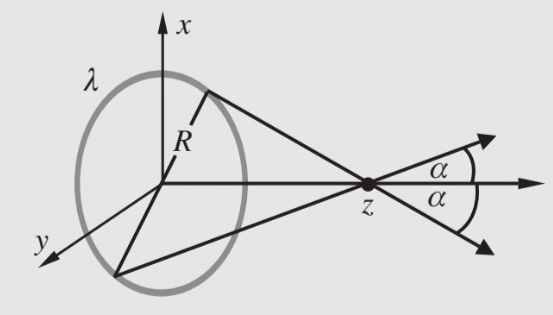
\includegraphics[width=0.9\linewidth,height=0.6\linewidth]{3p1.png}
}%
}
\end{center}
\end{columns}
\end{frame}

%------------------------------------------------
\begin{frame}{Campo no eixo de um anel}
\begin{eqbox}
\begin{equation}
\E_{\text{anel}}(z\ge 0)=
\frac{\lambda}{4\pi\epsilon_0}
\oint d\ell\;
\frac{\cos\alpha}{z^2+R^2}\,\zhat
\label{eq:3.10a}
\end{equation}
\end{eqbox}

\vspace{0.15cm}

\begin{eqbox}
\begin{equation}
\E_{\text{anel}}(z\ge 0)=
\frac{\lambda}{4\pi\epsilon_0}
\frac{2\pi R z}{(z^2+R^2)^{3/2}}\,
\zhat
=
\frac{Q}{4\pi\epsilon_0}
\frac{z}{(z^2+R^2)^{3/2}}\,
\zhat
\label{eq:3.10b}
\end{equation}
\end{eqbox}

\vspace{0.2cm}

\begin{block}{Observações}
\begin{itemize}
    \item Em \(z=0\), o campo é nulo por simetria.
    \item Para \(z\gg R\), recuperamos o comportamento de uma carga puntiforme total \(Q\).
\end{itemize}
\end{block}
\end{frame}

%------------------------------------------------
\begin{frame}{Disco uniformemente carregado}
\begin{mybox}
\justifying
O disco pode ser visto como uma superposição de anéis concêntricos de raio \(r\), cada um contendo
\[
dQ=2\pi r \sigma\,dr.
\]
Somando as contribuições de todos esses anéis, obtemos o campo ao longo do eixo.
\end{mybox}

\vspace{0.2cm}

\begin{eqbox}
\begin{equation}
\E_{\text{disco}}(z>0)=
\frac{z}{4\pi\epsilon_0}
\int_{0}^{R}dr\;
\frac{2\pi r\sigma}{(z^2+r^2)^{3/2}}\,\zhat
\label{eq:3.10c}
\end{equation}
\end{eqbox}

\vspace{0.15cm}

\begin{eqbox}
\begin{equation}
\E_{\text{disco}}(z>0)=
\frac{\sigma}{2\epsilon_0}
\left(
1-\frac{z}{\sqrt{z^2+R^2}}
\right)\zhat
\label{eq:3.10d}
\end{equation}
\end{eqbox}
\end{frame}

%------------------------------------------------
\begin{frame}{Limite de folha infinita e condição de salto}
\begin{eqbox}
\begin{equation}
\lim_{R\to\infty}\E_{\text{disco}}(z>0)
=
\E_{\text{folha}}(z>0)
=
\frac{\sigma}{2\epsilon_0}\,\zhat
\label{eq:3.10e}
\end{equation}
\end{eqbox}

\vspace{0.2cm}

\begin{mybox}
\justifying
Por simetria, no lado oposto da folha,
\[
\E(z<0)=-\E(z>0).
\]
Logo, a componente normal do campo sofre uma descontinuidade ao atravessar a superfície carregada.
\end{mybox}

\vspace{0.15cm}

\begin{eqbox}
\begin{equation}
\E(0^+)-\E(0^-)=\frac{\sigma}{\epsilon_0}\,\zhat
\label{eq:3.10f}
\end{equation}
\end{eqbox}

\vspace{0.15cm}

\begin{alertblock}{Mensagem física}
Uma camada superficial de carga produz um \textbf{salto finito} na componente normal do campo elétrico.
\end{alertblock}
\end{frame}

%------------------------------------------------
\begin{frame}{3.3 O potencial escalar}
\begin{mybox}
\justifying
A forma integral do campo em \eqref{eq:3.8} é poderosa, mas nem sempre fácil de calcular diretamente.
A estrutura de \eqref{eq:3.6} sugere definir uma nova função escalar, o \alert{potencial eletrostático}.
\end{mybox}

\vspace{0.2cm}

\begin{eqbox}
\begin{equation}
\varphi(\rr)=
\frac{1}{4\pi\epsilon_0}
\int d^3r'\,
\frac{\rho(\rr')}{\abs{\rr-\rr'}}
\label{eq:3.10}
\end{equation}
\end{eqbox}

\vspace{0.15cm}

\begin{eqbox}
\begin{equation}
\E(\rr)=-\nabla\varphi(\rr)
\label{eq:3.11}
\end{equation}
\end{eqbox}

\vspace{0.15cm}

\begin{block}{Vantagem conceitual}
\justifying
Em muitos problemas, é mais simples primeiro encontrar um escalar \(\varphi\) e depois obter \(\E\) por derivação, do que calcular diretamente uma integral vetorial.
\end{block}
\end{frame}

%------------------------------------------------
\begin{frame}{Casos particulares do potencial}
\begin{columns}[T,onlytextwidth]
\column{0.49\textwidth}
\begin{block}{Distribuição superficial}
Se toda a carga estiver sobre uma superfície, com densidade \(\sigma(\rr_s)\), então:
\begin{eqbox}
\begin{equation}
\varphi(\rr)=
\frac{1}{4\pi\epsilon_0}
\int dS\;
\frac{\sigma(\rr_s)}{\abs{\rr-\rr_s}}
\label{eq:3.12}
\end{equation}
\end{eqbox}
\end{block}

\column{0.49\textwidth}
\begin{block}{Distribuição linear}
Se toda a carga estiver confinada a um filamento, com densidade linear \(\lambda(\ell)\), então:
\begin{eqbox}
\begin{equation}
\varphi(\rr)=
\frac{1}{4\pi\epsilon_0}
\int d\ell\;
\frac{\lambda(\ell)}{\abs{\rr-\ell}}
\label{eq:3.13}
\end{equation}
\end{eqbox}
\end{block}
\end{columns}

\vspace{0.2cm}

\begin{mybox}
\justifying
Essas expressões são muito úteis em problemas com simetria planar, cilíndrica ou em geometrias reduzidas.
\end{mybox}
\end{frame}

%------------------------------------------------
\begin{frame}{Da lei de Gauss à equação de Poisson}
\begin{mybox}
\justifying
Aplicando a divergência à relação \(\E=-\nabla\varphi\) e usando a lei de Gauss, obtemos a equação fundamental para o potencial eletrostático.
\end{mybox}

\vspace{0.2cm}

\begin{eqbox}
\begin{equation}
\nabla^2\varphi(\rr)=-\frac{\rho(\rr)}{\epsilon_0}
\label{eq:3.14}
\end{equation}
\end{eqbox}

\vspace{0.2cm}

\begin{block}{Interpretação}
\begin{itemize}
    \item \textbf{Poisson}: quando há fontes, \(\rho(\rr)\neq 0\).
    \item \textbf{Laplace}: quando a região é livre de carga, \(\rho(\rr)=0\), de modo que
    \[
    \nabla^2\varphi=0.
    \]
\end{itemize}
\end{block}

\end{frame}

\begin{frame}

\begin{alertblock}{Importância}
Grande parte da eletrostática prática se reduz a resolver a equação de Poisson ou, em regiões sem carga, a equação de Laplace.
\end{alertblock}
\end{frame}

%------------------------------------------------
\begin{frame}{Exemplo 3.2: mudança de escala na distribuição}
\begin{block}{Hipótese}
\justifying
Considere duas distribuições de carga com a mesma forma geométrica, mas em escalas diferentes:
\[
\rho_B(\rr)=\lambda\,\rho_A(\lambda \rr),
\]
onde \(\lambda\) é constante.
\end{block}

\vspace{0.2cm}

\begin{mybox}
\justifying
Queremos relacionar:
\begin{itemize}
    \item os potenciais \(\varphi_A(\rr)\) e \(\varphi_B(\rr)\);
    \item os campos \(\E_A(\rr)\) e \(\E_B(\rr)\).
\end{itemize}
O truque é reescalar a variável de integração na definição do potencial.
\end{mybox}

\end{frame}

\begin{frame}

\begin{center}
\fbox{%
\parbox[c][3.5cm][c]{0.95\linewidth}{%
\centering
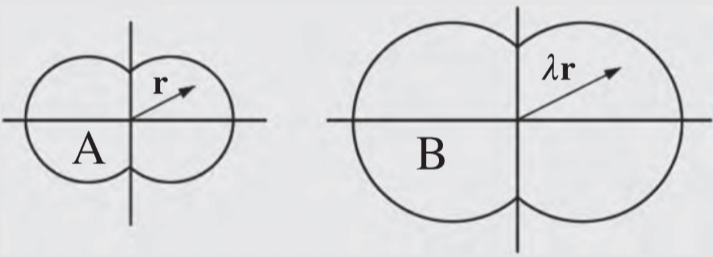
\includegraphics[width=0.8\linewidth]{3p2.png}
}%
}
\end{center}
\end{frame}

%------------------------------------------------
\begin{frame}{Resultado da mudança de escala}

Usando a dica:
\begin{eqbox}
\begin{equation}
\varphi_A(\mathbf{r})
=
\frac{1}{4\pi\epsilon_0}
\int d^3 r'\,
\frac{\rho_A(\mathbf{r}')}{\lvert \mathbf{r}-\mathbf{r}' \rvert}
=
\frac{1}{4\pi\epsilon_0}
\int d^3 r'\,
\frac{\rho_B(\lambda \mathbf{r}')}{\lvert \mathbf{r}-\mathbf{r}' \rvert}
\label{eq:ex3.2a}
\end{equation}
\end{eqbox}

\vspace{0.2cm}

Trocando a variável de integração para $\lambda \mathbf{r}'$
\begin{eqbox}
\begin{equation}
\varphi_A(\mathbf{r})
=
\frac{1}{4\pi\epsilon_0}
\frac{1}{\lambda^2}
\int d^3(\lambda \mathbf{r}')\,
\frac{\rho_B(\lambda \mathbf{r}')}{\lvert \lambda \mathbf{r}-\lambda \mathbf{r}' \rvert}
=
\frac{1}{\lambda^2}\,
\varphi_B(\lambda \mathbf{r})
\label{eq:ex3.2b}
\end{equation}
\end{eqbox}

\vspace{0.2cm}
$\text{Então, como } \mathbf{E} = -\nabla \varphi$,
\begin{eqbox}
\begin{equation}
\mathbf{E}_B(\lambda \mathbf{r})
=
-\,\frac{\partial}{\partial(\lambda \mathbf{r})}\,
\varphi_B(\lambda \mathbf{r})
=
-\,\frac{\partial}{\partial(\lambda \mathbf{r})}\,
\lambda^2 \varphi_A(\mathbf{r})
=
\lambda\,\mathbf{E}_A(\mathbf{r})
\label{eq:ex3.2c}
\end{equation}
\end{eqbox}

\end{frame}

\begin{frame}

\begin{block}{Leitura física}
\justifying
Ao reescalar o tamanho da distribuição, o potencial e o campo não mudam da mesma maneira:
\begin{itemize}
    \item o potencial ganha um fator \(1/\lambda^2\);
    \item o campo transforma-se linearmente com \(\lambda\).
\end{itemize}
\end{block}
\end{frame}

%------------------------------------------------
\begin{frame}{3.3.1 A força de Coulomb é conservativa}
\begin{mybox}
\justifying
Como \(\E=-\nabla\varphi\), o trabalho realizado pela força elétrica sobre uma carga puntiforme \(q\) entre dois pontos depende apenas dos valores do potencial nos extremos.
\end{mybox}

\vspace{0.2cm}

\begin{eqbox}
\begin{equation}
W_e[\rr_1\to \rr_2]
=
q\int_{\rr_1}^{\rr_2} d\ell\cdot \E(\rr)
=
-q\int_{\rr_1}^{\rr_2} d\ell\cdot \nabla\varphi
=
-q\,[\varphi(\rr_2)-\varphi(\rr_1)]
\label{eq:3.15}
\end{equation}
\end{eqbox}

\vspace{0.2cm}

\begin{alertblock}{Conclusão}
\justifying
O trabalho não depende do caminho seguido, mas apenas dos pontos inicial e final. 
Isso caracteriza a força eletrostática como \textbf{conservativa}.
\end{alertblock}
\end{frame}

%------------------------------------------------
\begin{frame}{Trabalho em um caminho fechado}
\begin{columns}[T,onlytextwidth]
\column{0.55\textwidth}
\begin{eqbox}
\begin{equation}
W_{\text{ciclo}}
=
q\oint_C d\ell\cdot \E
=
q\int_S d\mathbf{S}\cdot \nabla\times \E
=
0
\label{eq:3.16}
\end{equation}
\end{eqbox}

\vspace{0.2cm}

\begin{block}{Interpretação}
\justifying
Como \(\nabla\times \E=0\), o trabalho ao percorrer qualquer curva fechada \(C\) é nulo.
Isso equivale à independência do caminho e reforça a natureza conservativa da força de Coulomb.
\end{block}

\column{0.40\textwidth}
\begin{center}
\fbox{%
\parbox[c][4.7cm][c]{0.92\linewidth}{%
\centering
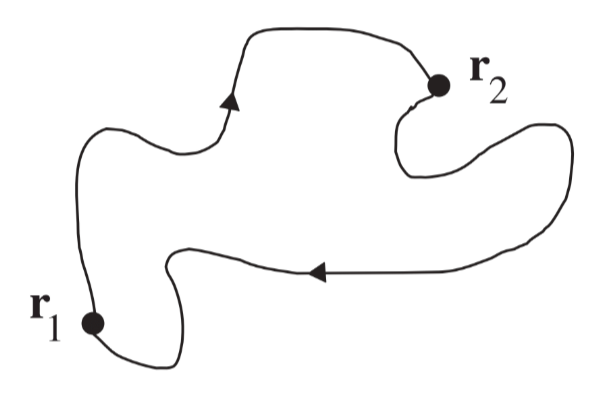
\includegraphics[width=0.9\linewidth,height=0.6\linewidth]{3p3.png}
}%
}
\end{center}
\end{columns}
\end{frame}

%------------------------------------------------
\begin{frame}{Diferença de potencial e escolha do zero}
\begin{mybox}
\justifying
O potencial é definido a menos de uma constante aditiva. 
Por isso, podemos escolher arbitrariamente um ponto de referência \(\rr_0\) onde o potencial é fixado.
\end{mybox}


\begin{eqbox}
\begin{equation}
\varphi(\rr)-\varphi(\rr_0)
=
-\int_{\rr_0}^{\rr} d\ell\cdot \E
\label{eq:3.17}
\end{equation}
\end{eqbox}

\vspace{0.05cm}

\begin{eqbox}
\begin{equation}
\varphi(\rr)=
-\int_{\rr_0}^{\rr} d\ell\cdot \E
\qquad \text{se } \varphi(\rr_0)=0
\label{eq:3.18}
\end{equation}
\end{eqbox}

\vspace{0.05cm}

\begin{block}{Escolha usual}
Para distribuições localizadas, é comum adotar
\[
\varphi(\infty)=0.
\]
\end{block}
\end{frame}

%------------------------------------------------
\begin{frame}{Resumo conceitual do capítulo (1/2)}
\begin{mybox}
\begin{enumerate}
    \item A eletrostática é governada por
    \[
    \nabla\times \E=0,
    \qquad
    \epsilon_0\nabla\cdot\E=\rho.
    \]

    \item A lei de Coulomb em forma integral é
    \[
    \E(\rr)=\frac{1}{4\pi\epsilon_0}\int d^3r'\,\rho(\rr')\frac{\rr-\rr'}{\abs{\rr-\rr'}^3}.
    \]

    \item O potencial escalar simplifica a teoria:
    \[
    \E=-\nabla\varphi.
    \]
\end{enumerate}
\end{mybox}
\end{frame}

%------------------------------------------------

\begin{frame}{Resumo conceitual do capítulo (2/2)}
\begin{mybox}
\begin{enumerate}
    \setcounter{enumi}{3}

    \item O potencial satisfaz a equação de Poisson:
    \[
    \nabla^2\varphi=-\frac{\rho}{\epsilon_0}.
    \]

    \item A força de Coulomb é conservativa:
    \[
    \oint_C d\ell\cdot \E=0.
    \]
\end{enumerate}
\end{mybox}
\end{frame}


\begin{frame}{Exercício 3.2: Simétrico e sem traço}

\begin{block}{}
As componentes cartesianas do campo elétrico em uma região livre de cargas são
\[
E_k = C_k + D_{jk}\, r_j,
\]
onde \(C_k\) e \(D_{jk}\) são constantes.
\end{block}


\begin{mybox}
\begin{enumerate}
    \item[(a)] Mostre que \(D_{jk}\) é \textbf{simétrico}
    \[
    D_{jk}=D_{kj}
    \]
    e \textbf{sem traço}
    \[
    \sum_k D_{kk}=0.
    \]


    \item[(b)] Encontre o \textbf{potencial eletrostático mais geral}
    que gera o campo elétrico do item (a).
\end{enumerate}
\end{mybox}

\end{frame}


%------------------------------------------------
\begin{frame}{Por que esse exercício existe?}

\begin{mybox}
\justifying
O campo dado
\[
E_k = C_k + D_{jk} r_j
\]
não é arbitrário: ele representa a \alert{expansão de Taylor} do campo elétrico em torno de um ponto.
\end{mybox}

\vspace{0.2cm}

\begin{eqbox}
\begin{equation}
\mathbf{E}(\mathbf{r})
\approx
\mathbf{E}(0)
+
(\nabla \mathbf{E})\cdot \mathbf{r}
\end{equation}
\end{eqbox}

\vspace{0.2cm}

\begin{block}{Interpretação}
\begin{itemize}
    \item \(C_k\) = campo uniforme (ordem zero)
    \item \(D_{jk}\) = variação espacial do campo
\end{itemize}
\end{block}

\end{frame}

%------------------------------------------------
\begin{frame}{Significado físico do tensor \(D_{jk}\)}

\begin{eqbox}
\begin{equation}
D_{jk} = \frac{\partial E_k}{\partial r_j}
\end{equation}
\end{eqbox}

\vspace{0.2cm}

\begin{mybox}
\justifying
O tensor \(D_{jk}\) mede \alert{como o campo muda no espaço}.  
Ele contém toda a informação sobre \textbf{gradientes do campo elétrico}.
\end{mybox}

\vspace{0.2cm}

\begin{block}{Onde isso aparece na prática?}
\begin{itemize}
    \item Força sobre dipolos: \(\mathbf{F}=(\mathbf{p}\cdot\nabla)\mathbf{E}\)
    \item Armadilhas eletrostáticas (íons, elétrons)
    \item Interações quadrupolares em átomos
    \item Campos não uniformes em experimentos reais
\end{itemize}
\end{block}

\end{frame}

%------------------------------------------------
\begin{frame}{Por que \(D_{jk}\) deve ser simétrico?}

\begin{eqbox}
\begin{equation}
\nabla \times \mathbf{E} = 0
\end{equation}
\end{eqbox}

\vspace{0.2cm}

\begin{mybox}
\justifying
Em eletrostática, o campo não pode ter rotação local.
Isso impõe:
\[
D_{jk} = D_{kj}
\]
\end{mybox}

\vspace{0.2cm}

\begin{alertblock}{Interpretação}
A parte antissimétrica corresponderia a uma \textbf{rotação local do campo}.  
Isso é proibido em eletrostática.
\end{alertblock}

\end{frame}

%------------------------------------------------
\begin{frame}{Por que \(D_{kk}=0\)?}

\begin{eqbox}
\begin{equation}
\nabla \cdot \mathbf{E} = 0
\end{equation}
\end{eqbox}

\vspace{0.2cm}

\begin{mybox}
\justifying
Em uma região sem carga, o campo não pode ter fontes nem sumidouros.
Isso implica:
\[
D_{kk} = 0
\]
\end{mybox}

\vspace{0.2cm}

\begin{alertblock}{Interpretação}
O traço mede o quanto o campo está \textbf{expandindo ou comprimindo volume}.  
Sem carga → volume preservado → traço zero.
\end{alertblock}

\end{frame}

%------------------------------------------------
\begin{frame}{Interpretação geométrica}

\begin{mybox}
\justifying
O tensor \(D_{jk}\) descreve como o campo \alert{deforma o espaço localmente}.
\end{mybox}

\vspace{0.2cm}

\begin{block}{Decomposição}
\begin{itemize}
    \item Parte antissimétrica → rotação (proibida)
    \item Parte com traço → fonte/sumidouro (proibida)
    \item Resta: deformação pura (permitida)
\end{itemize}
\end{block}

\vspace{0.2cm}

\begin{alertblock}{Analogia poderosa}
Isso é análogo a:
\begin{itemize}
    \item tensor de deformação (elasticidade)
    \item tensor de maré (gravitação)
\end{itemize}
\end{alertblock}

\end{frame}

%------------------------------------------------
\begin{frame}{Conexão com o potencial}

\begin{eqbox}
\begin{equation}
\mathbf{E} = -\nabla \varphi
\end{equation}
\end{eqbox}

\vspace{0.2cm}

\begin{eqbox}
\begin{equation}
D_{jk} = -\partial_j \partial_k \varphi
\end{equation}
\end{eqbox}


\begin{mybox}
\justifying
O tensor \(D_{jk}\) é o \alert{Hessiano do potencial}.
\end{mybox}


\begin{eqbox}
\begin{equation}
\nabla^2 \varphi = 0
\end{equation}
\end{eqbox}


\begin{alertblock}{Mensagem central}
O traço nulo de \(D\) é exatamente a equação de Laplace.
\end{alertblock}

\end{frame}

%------------------------------------------------
\begin{frame}{Mensagem final do exercício}

\begin{mybox}
\justifying
Este exercício mostra que o campo eletrostático mais geral, localmente, é:
\end{mybox}


\begin{eqbox}
\begin{equation}
\mathbf{E}(\mathbf{r})
=
\text{campo uniforme}
+
\text{deformação linear (sem rotação e sem fonte)}
\end{equation}
\end{eqbox}


\begin{block}{Ideia profunda}
\begin{itemize}
    \item Maxwell → restrições físicas
    \item restrições → estrutura matemática
    \item estrutura → forma do campo
\end{itemize}
\end{block}


\begin{alertblock}{Resumo em uma frase}
O tensor \(D_{jk}\) é o gradiente do campo elétrico, e sua forma é totalmente determinada pelas equações de Maxwell.
\end{alertblock}

\end{frame}


\begin{frame}{Exercício 3.5: Lei de Gauss na prática}

\begin{block}{}
Utilize a \alert{lei de Gauss} para determinar o campo elétrico quando a densidade de carga é:
\end{block}


\begin{mybox}
\small
\begin{enumerate}
    \item[(a)] 
    \[
    \rho(x) = \rho_0\, e^{-\kappa \sqrt{x^2}}.
    \]
    Expresse a resposta em \textbf{coordenadas cartesianas}.

    \vspace{0.2cm}

    \item[(b)] 
    \[
    \rho(x,y) = \rho_0\, e^{-\kappa \sqrt{x^2 + y^2}}.
    \]
    Expresse a resposta em \textbf{coordenadas cilíndricas}.


    \item[(c)] 
    \[
    \rho(x,y,z) = \rho_0\, e^{-\kappa \sqrt{x^2 + y^2 + z^2}}.
    \]
    Expresse a resposta em \textbf{coordenadas esféricas}.
\end{enumerate}
\end{mybox}


\begin{alertblock}{Dica}
Identifique a \textbf{simetria do problema} antes de aplicar a lei de Gauss:
planar, cilíndrica ou esférica.
\end{alertblock}

\end{frame}


\begin{frame}{Distribuições de carga}

\begin{center}
\begin{columns}[c,onlytextwidth]

\column{0.33\textwidth}
\begin{mybox}
\centering
\textbf{(a)}\\[2mm]
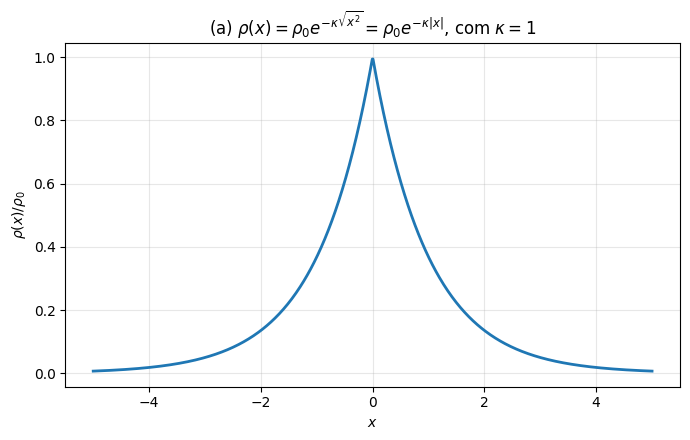
\includegraphics[width=\linewidth]{a.png}
\end{mybox}

\column{0.33\textwidth}
\begin{mybox}
\centering
\textbf{(b)}\\[2mm]
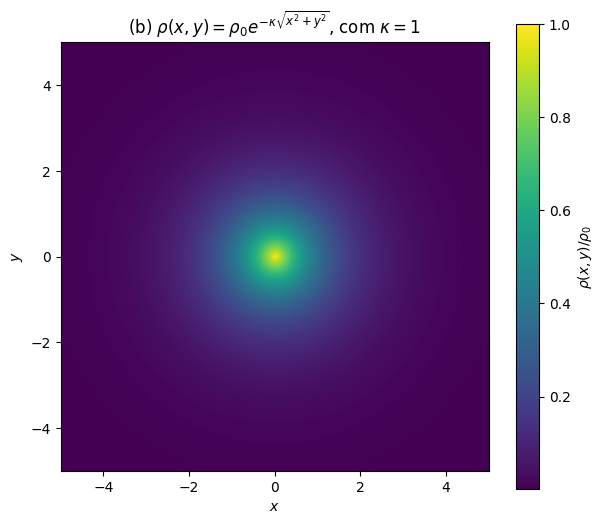
\includegraphics[width=\linewidth]{b.png}
\end{mybox}

\column{0.33\textwidth}
\begin{mybox}
\centering
\textbf{(c)}\\[2mm]
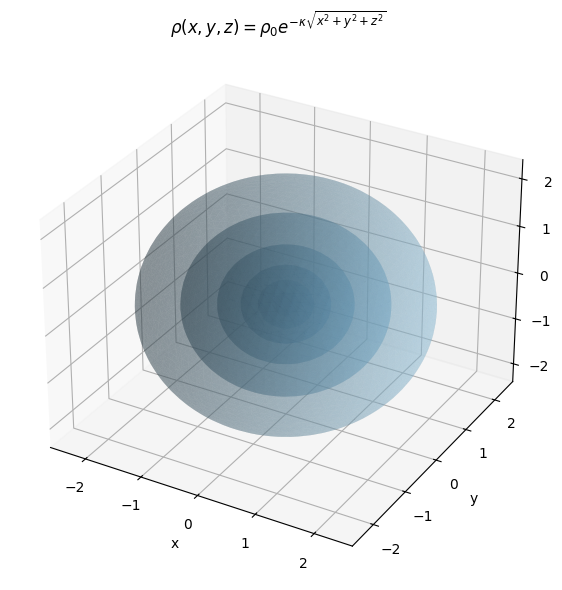
\includegraphics[width=\linewidth]{c.png}
\end{mybox}

\end{columns}
\end{center}

\end{frame}

\begin{frame}{Plots das Soluções}
    
\begin{center}
\begin{columns}[c,onlytextwidth]

\column{0.33\textwidth}
\begin{mybox}
\centering
\textbf{(a)}\\[2mm]
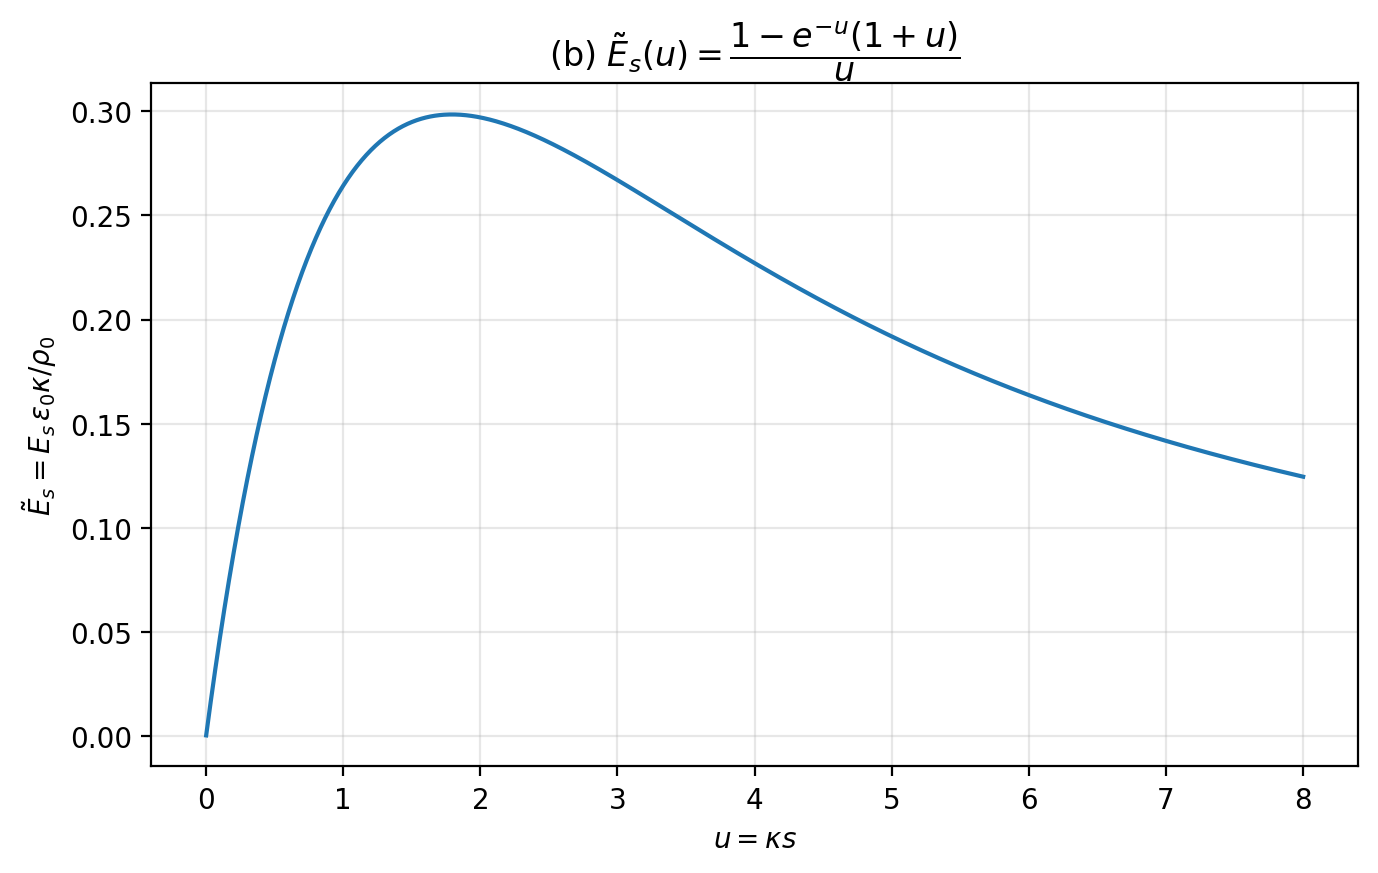
\includegraphics[width=\linewidth]{plot_campo_b.png}
\end{mybox}

\column{0.33\textwidth}
\begin{mybox}
\centering
\textbf{(b)}\\[2mm]
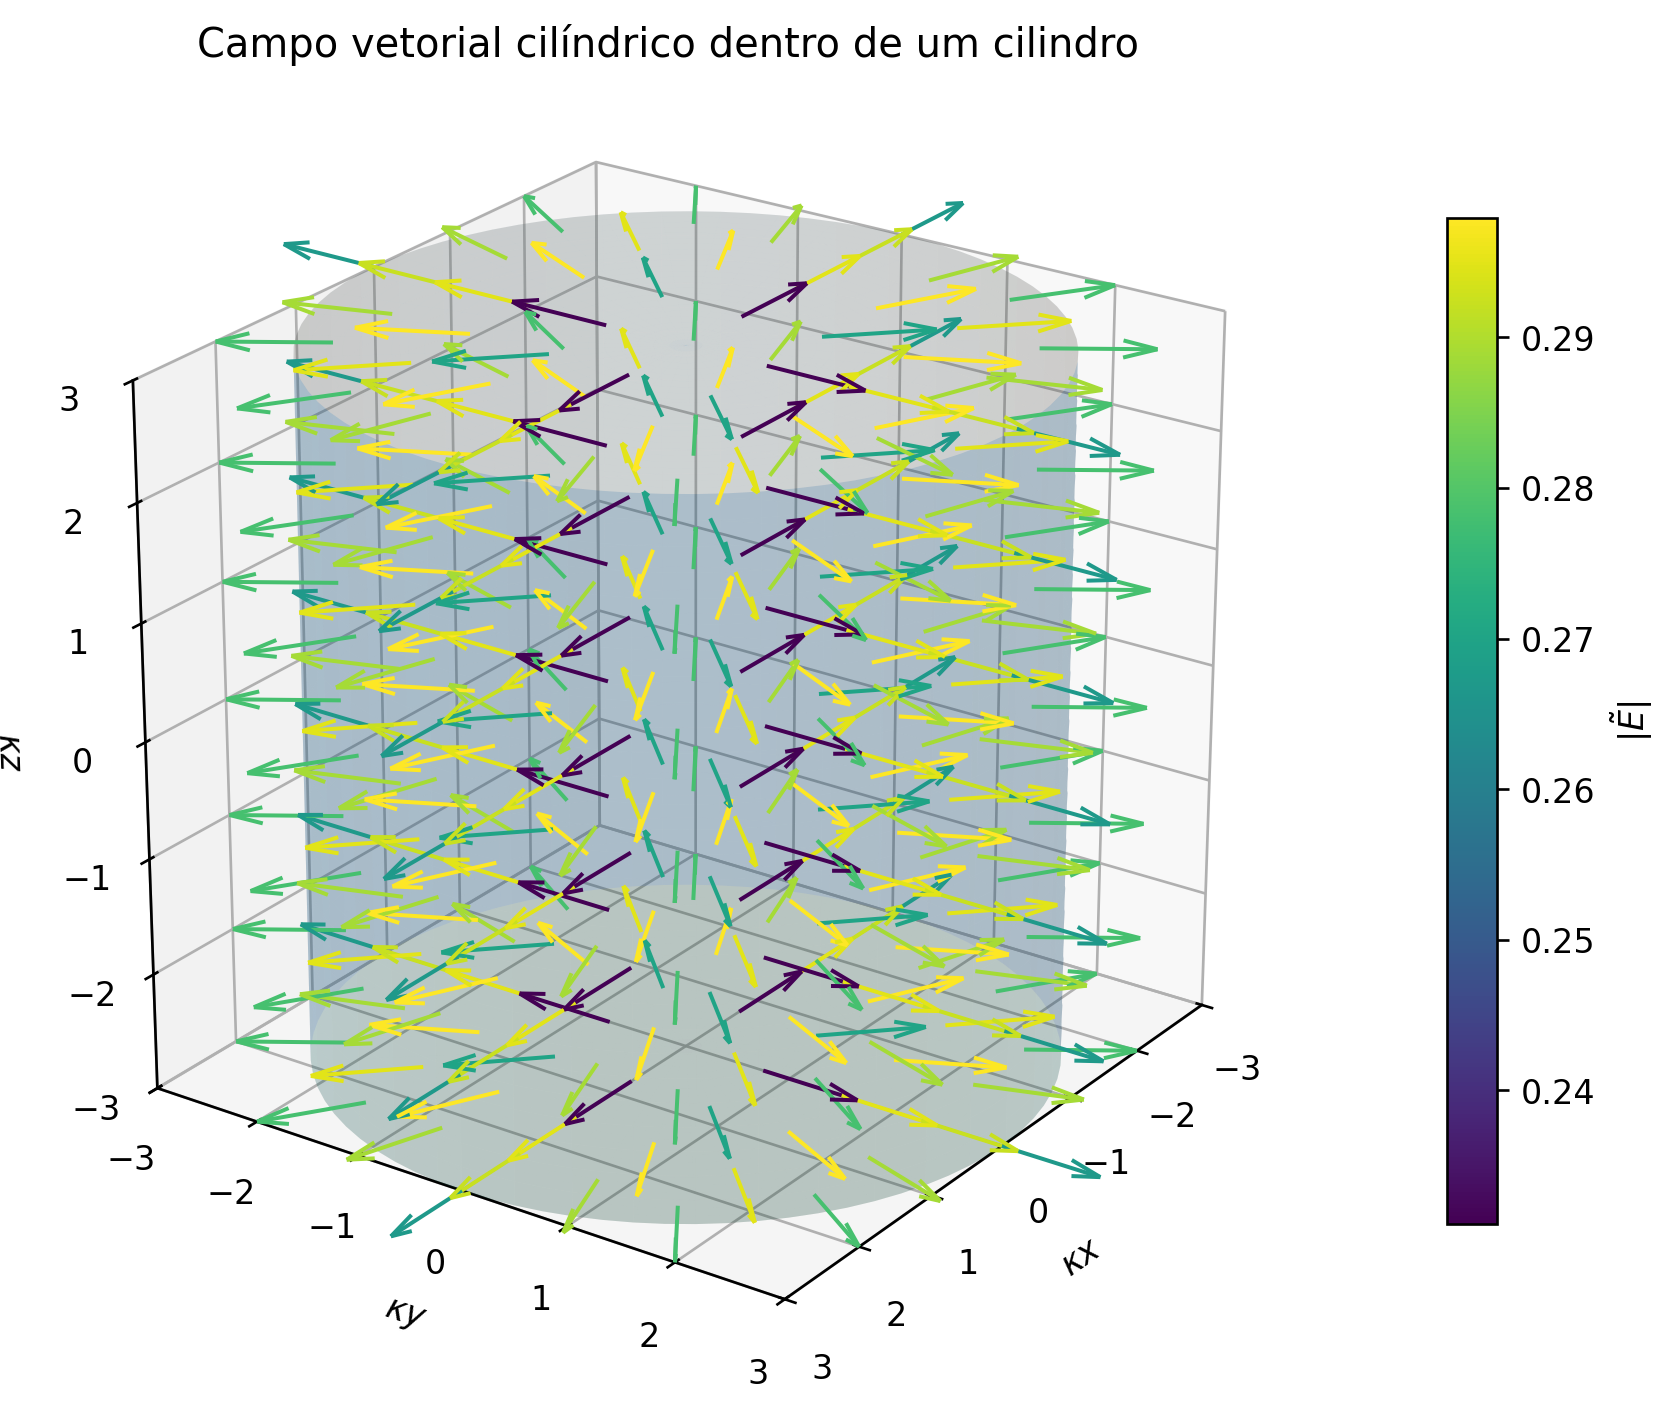
\includegraphics[width=\linewidth]{campo_cilindrico_cilindro_3D.png}
\end{mybox}

\column{0.33\textwidth}
\begin{mybox}
\centering
\textbf{(c)}\\[2mm]
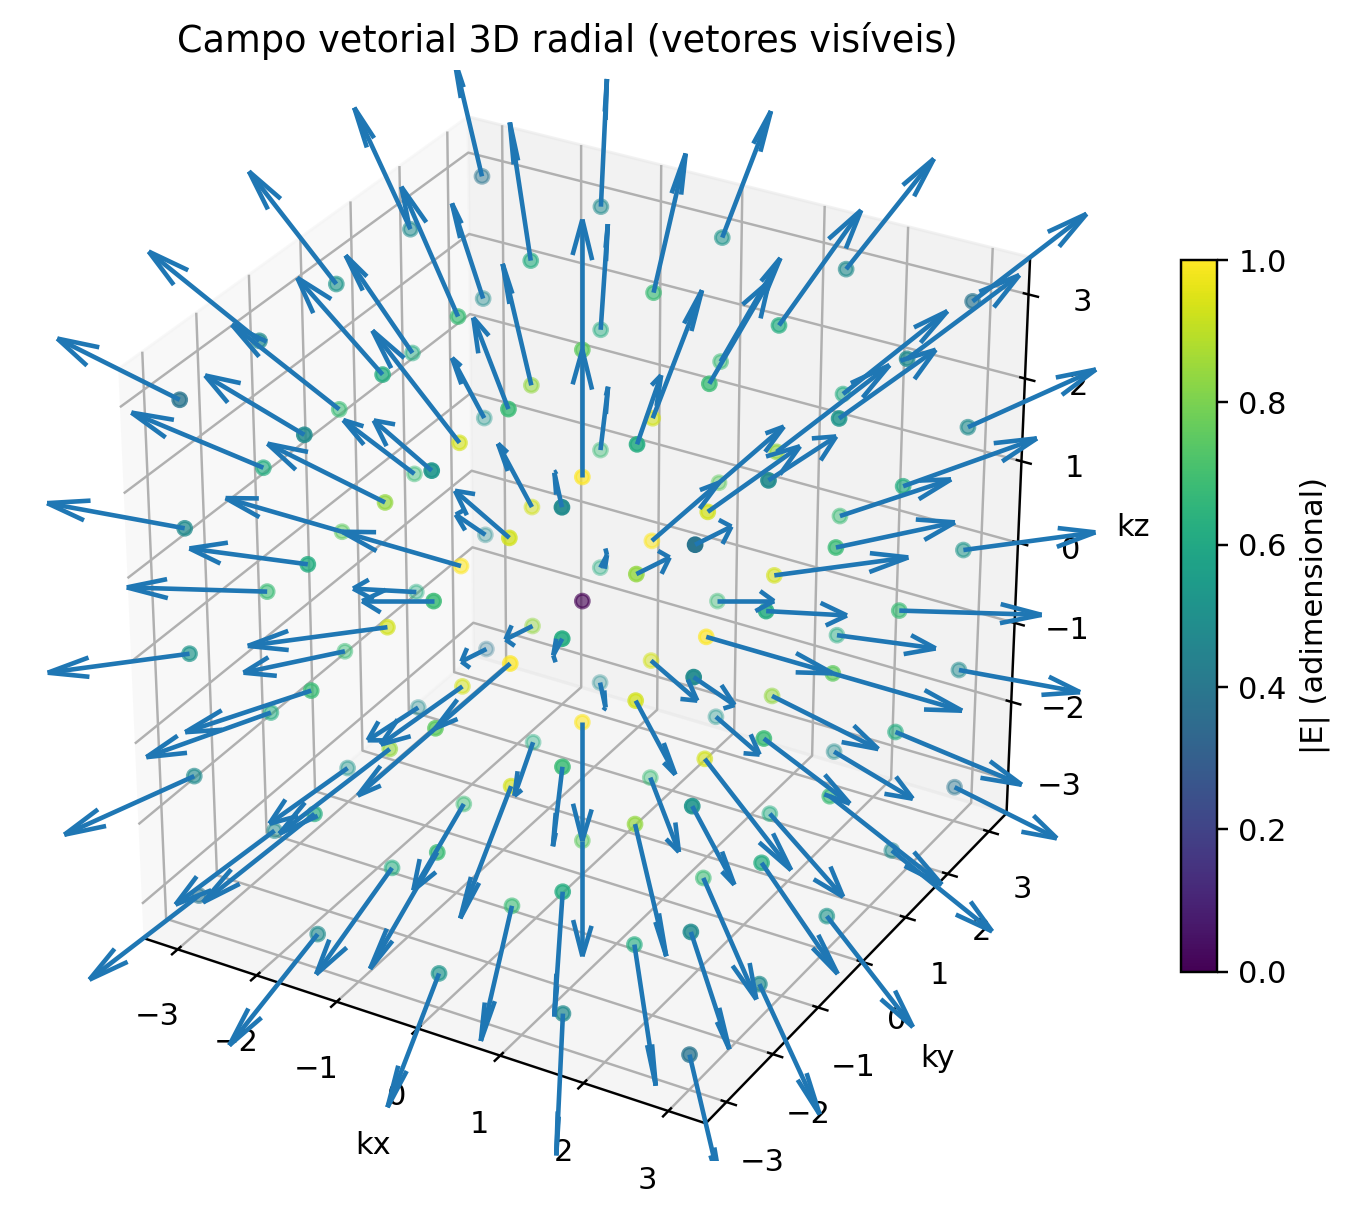
\includegraphics[width=\linewidth]{campo_c_vetorial_3D_grande.png}
\end{mybox}

\end{columns}
\end{center}
\end{frame}

\begin{frame}{3.3.2 Condições de contorno para $\phi(\mathbf{r})$}
\begin{block}{Ideia física}
As condições de contorno do potencial eletrostático decorrem do comportamento do campo elétrico próximo a uma interface com densidade de carga superficial $\sigma(\mathbf{r}_S)$.
\end{block}

\begin{itemize}
\item Seja $\hat{\mathbf{n}}_2$ o vetor normal saindo da região 2;
\item Definimos a derivada direcional:
\begin{equation}
\frac{\partial}{\partial n_2} = \hat{\mathbf{n}}_2 \cdot \nabla
\end{equation}
\item Sabemos que:
\begin{equation}
\mathbf{E} = -\nabla \phi
\end{equation}
\end{itemize}
\end{frame}

%-------------------------------------------------

\begin{frame}{Descontinuidade do campo elétrico normal}
\begin{block}{Condição de contorno para $\mathbf{E}$}
\begin{equation}
\hat{\mathbf{n}}_2 \cdot (\mathbf{E}_1 - \mathbf{E}_2) = \frac{\sigma}{\epsilon_0}
\end{equation}
\end{block}

\pause

Substituindo $\mathbf{E} = -\nabla \phi$:

\begin{equation}
\hat{\mathbf{n}}_2 \cdot \left(-\nabla \phi_1 + \nabla \phi_2\right) = \frac{\sigma}{\epsilon_0}
\end{equation}

\pause

\begin{alertblock}{Resultado}
\begin{equation}
\left[
\frac{\partial \phi_2}{\partial n_2}
-
\frac{\partial \phi_1}{\partial n_2}
\right]
=
\frac{\sigma}{\epsilon_0}
\tag{3.19}
\end{equation}
\end{alertblock}

\end{frame}

%-------------------------------------------------

\begin{frame}{Interpretação física}
\begin{itemize}
\item A derivada normal do potencial sofre uma \textbf{descontinuidade};
\item Essa descontinuidade é causada pela presença de \textbf{carga superficial};
\item Ou seja:
\begin{center}
\textit{o campo elétrico normal é descontínuo na interface}
\end{center}
\end{itemize}

\pause

\begin{block}{Resumo}
\begin{equation}
\boxed{
\text{salto na derivada normal de } \phi \;\Longleftrightarrow\; \sigma \neq 0
}
\end{equation}
\end{block}
\end{frame}

%-------------------------------------------------

\begin{frame}{Continuidade do potencial}
\begin{block}{Argumento físico}
Considere dois pontos infinitesimalmente próximos em lados opostos da interface.
\end{block}

\pause

\begin{itemize}
\item A separação $|\mathbf{r} - \mathbf{r}_0| \to 0$;
\item A integral relevante só pode ser não nula se $\mathbf{E}$ divergir;
\item Porém:
\begin{center}
$\mathbf{E}$ é finito (exceto na componente normal já tratada)
\end{center}
\end{itemize}

\pause

\begin{alertblock}{Conclusão}
O potencial é contínuo ao atravessar a interface.
\end{alertblock}
\end{frame}

%-------------------------------------------------

\begin{frame}{Condição de continuidade}
\begin{equation}
\phi_1(\mathbf{r}_S) = \phi_2(\mathbf{r}_S)
\tag{3.20}
\end{equation}

\pause

\begin{block}{Interpretação}
\begin{itemize}
\item O potencial não pode ter saltos finitos;
\item Caso contrário:
\begin{itemize}
\item $\nabla \phi$ teria uma divergência infinita;
\item implicaria $\mathbf{E} \to \infty$ (não físico).
\end{itemize}
\end{itemize}
\end{block}

\end{frame}


%-------------------------------------------------
\begin{frame}{Continuidade do potencial: PROVA}
\begin{block}{Queremos provar}
\begin{equation}
\phi_1(\mathbf r_S)=\phi_2(\mathbf r_S)
\tag{3.20}
\end{equation}
\end{block}

\pause

\begin{itemize}
\item Consideramos dois pontos infinitamente próximos da interface:
\begin{itemize}
\item $\mathbf r_- = \mathbf r_S - \epsilon \hat{\mathbf n}$
\item $\mathbf r_+ = \mathbf r_S + \epsilon \hat{\mathbf n}$
\end{itemize}

\item Vamos analisar:
\begin{equation}
\phi(\mathbf r_+) - \phi(\mathbf r_-)
\end{equation}
\end{itemize}
\end{frame}

%-------------------------------------------------
\begin{frame}{Diferença de potencial como integral}
\begin{block}{Definição fundamental}
\begin{equation}
\phi(\mathbf r_+) - \phi(\mathbf r_-)
=
-\int_{\mathbf r_-}^{\mathbf r_+} \mathbf E \cdot d\mathbf l
\end{equation}
\end{block}

\pause

Escolhendo um caminho normal à superfície:

\begin{equation}
d\mathbf l = \hat{\mathbf n}\, dn
\end{equation}

\pause

\begin{equation}
\Rightarrow
\phi(\mathbf r_+) - \phi(\mathbf r_-)
=
-\int_{-\epsilon}^{+\epsilon} E_n(n)\, dn
\end{equation}

\begin{center}
onde $E_n = \mathbf E \cdot \hat{\mathbf n}$
\end{center}
\end{frame}

%-------------------------------------------------
\begin{frame}{Comportamento do campo na interface}
\begin{block}{Condição conhecida}
\begin{equation}
E_{2n} - E_{1n} = \frac{\sigma}{\epsilon_0}
\end{equation}
\end{block}

\pause

\begin{itemize}
\item O campo pode ter \textbf{salto finito};
\item Mas \textbf{não diverge} como $1/\epsilon$;
\item Logo, existe uma constante $M$ tal que:
\begin{equation}
|E_n(n)| \le M
\end{equation}
\end{itemize}

\pause

\begin{alertblock}{Conclusão}
O campo é \textbf{limitado} na vizinhança da interface.
\end{alertblock}
\end{frame}

%-------------------------------------------------
\begin{frame}{Prova da continuidade}
\begin{block}{Estimativa}
\begin{equation}
|\phi(\mathbf r_+) - \phi(\mathbf r_-)| 
\le \int_{-\epsilon}^{+\epsilon} |E_n|\, dn
\end{equation}
\end{block}

\pause

\begin{equation}
\le \int_{-\epsilon}^{+\epsilon} M\, dn = 2M\epsilon
\end{equation}

\pause

\begin{equation}
\Rightarrow
|\phi(\mathbf r_+) - \phi(\mathbf r_-)| \to 0
\quad (\epsilon \to 0)
\end{equation}

\pause

\begin{alertblock}{Resultado}
\begin{equation}
\phi_1(\mathbf r_S)=\phi_2(\mathbf r_S)
\end{equation}
\end{alertblock}
\end{frame}

%-------------------------------------------------
\begin{frame}{Prova por absurdo (mais forte)}
\begin{block}{Suponha}
\begin{equation}
\phi_2 - \phi_1 = \Delta \phi \neq 0
\end{equation}
\end{block}

\pause

Então:

\begin{equation}
\frac{\Delta \phi}{2\epsilon}
\sim \frac{\partial \phi}{\partial n}
\end{equation}

\pause

Como $\mathbf E = -\nabla \phi$:

\begin{equation}
E_n \sim -\frac{\Delta \phi}{2\epsilon}
\end{equation}

\pause

\begin{alertblock}{Problema}
\begin{equation}
E_n \to \infty \quad (\epsilon \to 0)
\end{equation}
\end{alertblock}

\pause

\begin{center}
\textbf{Isso não é físico para $\sigma$ finita!}
\end{center}
\end{frame}

%-------------------------------------------------
\begin{frame}{Interpretação via equação de Poisson}
\begin{block}{Equação fundamental}
\begin{equation}
\nabla^2 \phi = -\frac{\rho}{\epsilon_0}
\end{equation}
\end{block}

\pause

Para carga superficial:

\begin{equation}
\rho = \sigma \, \delta(n)
\end{equation}

\pause

\begin{equation}
\Rightarrow \nabla^2 \phi \sim \delta(n)
\end{equation}

\pause

\begin{itemize}
\item $\delta$ na \textbf{segunda derivada};
\item $\Rightarrow$ salto na \textbf{primeira derivada};
\item $\Rightarrow$ \textbf{$\phi$ permanece contínua}.
\end{itemize}
\end{frame}

%-------------------------------------------------
\begin{frame}{Resumo}
\begin{tcolorbox}[colback=black!5,colframe=black!80,title=Conclusão matemática]

\begin{equation}
\phi_1 = \phi_2
\end{equation}

\begin{equation}
\frac{\partial \phi_2}{\partial n}
-
\frac{\partial \phi_1}{\partial n}
=
\frac{\sigma}{\epsilon_0}
\end{equation}

\end{tcolorbox}

\pause

\begin{block}{Mensagem central}
\begin{center}
\textit{O potencial não pode ter salto finito, pois isso implicaria campo elétrico infinito.}
\end{center}
\end{block}

\end{frame}
%-------------------------------------------------

%-------------------------------------------------

\begin{frame}{Comentário importante}
\begin{block}{Relação com $\nabla \times \mathbf{E} = 0$}
\begin{itemize}
\item A existência de $\phi$ depende de:
\begin{equation}
\nabla \times \mathbf{E} = 0
\end{equation}

\item Isso implica:
\begin{itemize}
\item continuidade das componentes tangenciais de $\mathbf{E}$;
\item portanto, continuidade de $\phi$.
\end{itemize}
\end{itemize}
\end{block}

\pause

\begin{alertblock}{Insight}
As condições de contorno para $\phi$ carregam a mesma informação das condições para $\mathbf{E}$.
\end{alertblock}

\end{frame}



%-------------------------------------------------
\begin{frame}{3.3.3 Teorema de Earnshaw}
\begin{block}{}
O potencial eletrostático $\phi(\mathbf r)$ em uma região finita e livre de cargas $R$:

\begin{center}
\textbf{não possui máximos nem mínimos no interior}
\end{center}

\pause

\begin{center}
$\Rightarrow$ seus extremos ocorrem apenas na \textbf{fronteira}
\end{center}
\end{block}

\pause

\begin{alertblock}{Consequência física}
Não existe equilíbrio estável puramente eletrostático.
\end{alertblock}
\end{frame}

%-------------------------------------------------
\begin{frame}{Estratégia da prova}
\begin{block}{Ideia}
Vamos provar por \textbf{contradição}.
\end{block}

\pause

\begin{itemize}
\item Suponha que $\phi$ tenha um \textbf{mínimo local} em um ponto $P$;
\item Construímos uma pequena superfície fechada $S$ envolvendo $P$;
\item Analisamos o comportamento de $\nabla \phi$ nessa superfície.
\end{itemize}

\pause

\begin{center}
\textit{Se a hipótese levar a contradição, ela é falsa.}
\end{center}
\end{frame}

%-------------------------------------------------
\begin{frame}{Propriedade de um mínimo local}
\begin{block}{Se $\phi$ tem mínimo em $P$}
\begin{itemize}
\item $\phi(P)$ é menor que os valores ao redor;
\item Logo, ao sair de $P$, o potencial \textbf{aumenta}.
\end{itemize}
\end{block}

\pause

\begin{equation}
\hat{\mathbf n}\cdot \nabla \phi > 0
\end{equation}

\begin{center}
em toda a superfície $S$ ao redor de $P$
\end{center}

\pause

\begin{alertblock}{Interpretação}
O gradiente aponta \textbf{para fora} da superfície.
\end{alertblock}
\end{frame}

%-------------------------------------------------
\begin{frame}{Integral sobre a superfície}
\begin{equation}
\oint_S dS \; \hat{\mathbf n} \cdot \nabla \phi > 0
\tag{3.21}
\end{equation}

\pause

\begin{block}{Por quê?}
\begin{itemize}
\item $\hat{\mathbf n} \cdot \nabla \phi > 0$ em todos os pontos;
\item A integral de algo positivo continua positiva.
\end{itemize}
\end{block}
\end{frame}

%-------------------------------------------------
\begin{frame}{Usando o campo elétrico}
Sabemos que:

\begin{equation}
\mathbf E = -\nabla \phi
\end{equation}

\pause

Então:

\begin{equation}
\hat{\mathbf n}\cdot \mathbf E = -\hat{\mathbf n}\cdot \nabla \phi
\end{equation}

\pause

\begin{equation}
\Rightarrow
\oint_S dS \; \hat{\mathbf n}\cdot \mathbf E < 0
\end{equation}
\end{frame}

%-------------------------------------------------
\begin{frame}{Teorema da divergência}
\begin{block}{Transformando a integral}
\begin{equation}
\oint_S dS \; \hat{\mathbf n}\cdot \mathbf E
=
\int_V d^3r \; \nabla \cdot \mathbf E
\end{equation}
\end{block}

\pause

Logo:

\begin{equation}
\int_V d^3r \; \nabla \cdot \mathbf E < 0
\tag{3.22}
\end{equation}
\end{frame}

%-------------------------------------------------
\begin{frame}{Usando a equação de Maxwell}
Sabemos que:

\begin{equation}
\nabla \cdot \mathbf E = \frac{\rho}{\epsilon_0}
\end{equation}

\pause

Mas na região $R$:

\begin{equation}
\rho = 0
\end{equation}

\pause

\begin{equation}
\Rightarrow \nabla \cdot \mathbf E = 0
\end{equation}

\pause

\begin{equation}
\Rightarrow
\int_V d^3r \; \nabla \cdot \mathbf E = 0
\end{equation}
\end{frame}

%-------------------------------------------------
\begin{frame}{Contradição}
Obtivemos duas conclusões:

\begin{equation}
\int_V d^3r \; \nabla \cdot \mathbf E < 0
\end{equation}

\begin{equation}
\int_V d^3r \; \nabla \cdot \mathbf E = 0
\end{equation}

\pause

\begin{alertblock}{Contradição}
As duas não podem ser verdade simultaneamente.
\end{alertblock}

\pause

\begin{center}
$\Rightarrow$ A hipótese inicial é falsa.
\end{center}
\end{frame}

%-------------------------------------------------
\begin{frame}{Conclusão}
\begin{block}{Resultado}
\begin{itemize}
\item $\phi$ não pode ter \textbf{mínimos locais} no interior;
\item Um argumento idêntico mostra que não pode ter \textbf{máximos}.
\end{itemize}
\end{block}

\pause

\begin{equation}
\boxed{
\text{Os extremos de } \phi \text{ ocorrem apenas na fronteira}
}
\end{equation}

\pause

\begin{alertblock}{Interpretação física}
\begin{center}
Não existe aprisionamento eletrostático estável.
\end{center}
\end{alertblock}
\end{frame}

%-------------------------------------------------
\begin{frame}{Intuição física final}
\begin{itemize}
\item Linhas de campo elétrico:
\begin{itemize}
\item saem de cargas positivas;
\item entram em cargas negativas.
\end{itemize}

\pause

\item Em uma região sem cargas:
\begin{itemize}
\item não há fontes nem sumidouros;
\item o campo não pode "convergir" para um ponto.
\end{itemize}

\pause

\item Logo:
\begin{center}
não há como formar um mínimo ou máximo de potencial
\end{center}
\end{itemize}
\end{frame}


\begin{frame}{Exercício 3.10 — Dois Teoremas Eletrostáticos}

\begin{block}{}
\begin{enumerate}
\item[(a)] Use a segunda identidade de Green,
\begin{equation}
\int_V d^3r \,\big(f\nabla^2 g - g\nabla^2 f\big)
=
\oint_S d\mathbf{S}\cdot\big(f\nabla g - g\nabla f\big),
\end{equation}
para provar que o potencial $\phi(0)$ no centro de um volume esférico $V$, livre de cargas, é igual à média de $\phi(\mathbf r)$ sobre a superfície $S$ da esfera. 

\medskip

No texto, este teorema foi demonstrado usando a relação de reciprocidade de Green.

\medskip

\item[(b)] Use o resultado do item (a) para fornecer uma derivação alternativa do teorema de Earnshaw apresentado no texto.
\end{enumerate}
\end{block}

\end{frame}


\section{3.4 Gauss’ Law and Solid Angle}

\begin{frame}{Lei de Gauss (forma integral)}
\begin{eqbox}
\begin{equation}
\epsilon_0 \int_S d\mathbf S \cdot \mathbf E(\mathbf r) = Q_V
\tag{3.39}
\end{equation}
\end{eqbox}

\begin{itemize}
\item Relaciona fluxo elétrico com carga total envolvida.
\item Base para determinação de campos com simetria.
\item Independente da forma da superfície fechada.
\end{itemize}
\end{frame}

%-------------------------------------------------

\subsection{3.4.1 The Importance of Symmetry}

\begin{frame}{Importância da simetria}
\begin{mybox}{Ideia central}
Simetrias espaciais permitem determinar:
\begin{itemize}
\item direção do campo $\mathbf E$;
\item dependência funcional de sua magnitude;
\item escolha da superfície gaussiana ideal.
\end{itemize}
\end{mybox}

\pause
\begin{alertblock}{Ideia central}
Necessários para identificar uma superfície \(S\) na qual o termo \(d\mathbf{S}\cdot \mathbf{E}\) se reduz a uma quantidade escalar.
\end{alertblock}
\pause

\begin{itemize}
\item Rotacional, translacional, reflexão
\item Redução de integrais → escalares constantes
\end{itemize}
\end{frame}


\begin{frame}{Exemplos de Simetrias}

\begin{figure}
    \centering
    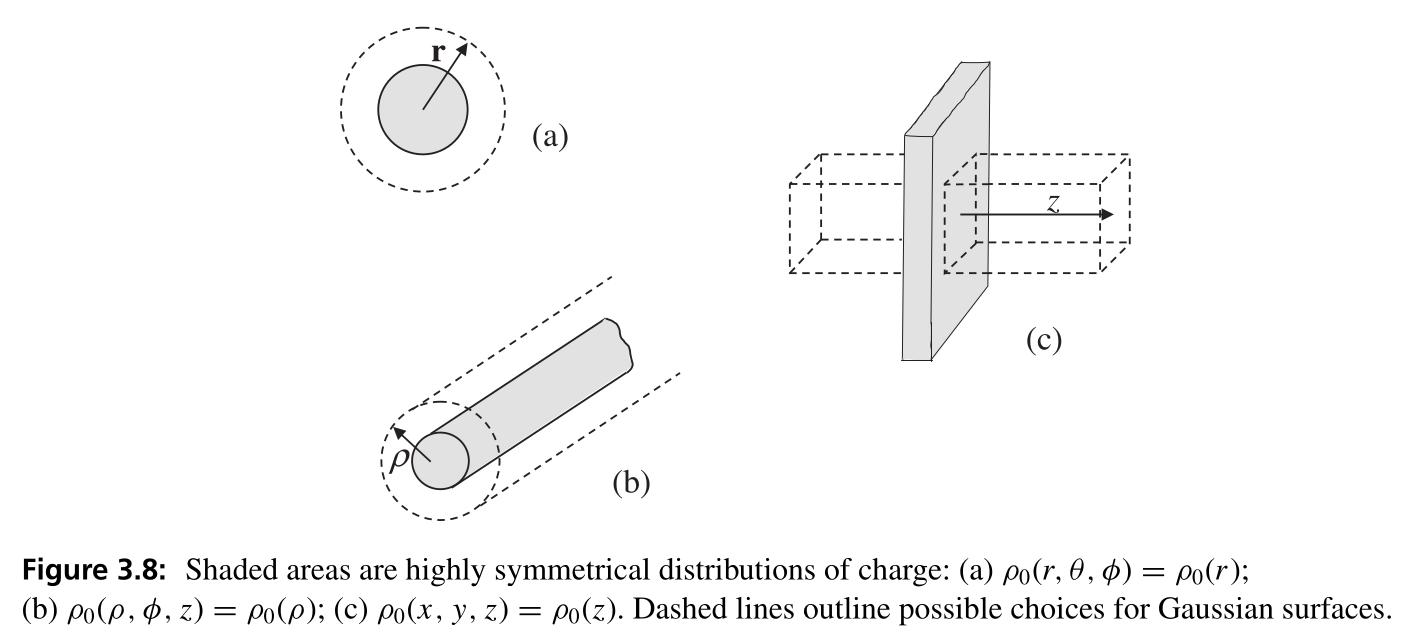
\includegraphics[width=0.8\linewidth]{3p8.png}
\end{figure}
    
\end{frame}
%-------------------------------------------------

\begin{frame}{Simetria esférica}
\begin{eqbox}
\begin{equation}
\mathbf E(r) = E(r)\,\hat{\mathbf r}
\quad \Rightarrow \quad
E(r) = \frac{Q(r)}{4\pi \epsilon_0 r^2}
\tag{3.40}
\end{equation}
\end{eqbox}

\begin{itemize}
\item Distribuição invariante por rotações
\item Campo puramente radial
\item Equivalente a carga pontual externa
\end{itemize}
\notas{pag. 1}
\end{frame}

%-------------------------------------------------

\begin{frame}{Potencial de carga pontual}
\begin{eqbox}
\begin{equation}
\varphi(r) = \frac{Q}{4\pi \epsilon_0 r}
\tag{3.41}
\end{equation}
\end{eqbox}

\begin{itemize}
\item Resultado direto da Lei de Gauss
\item Base para construção de soluções gerais
\end{itemize}
\notas{pag. 2}
\end{frame}

%-------------------------------------------------

\begin{frame}{Simetria cilíndrica}
\begin{eqbox}
\begin{equation}
\mathbf E(\rho) = E(\rho)\,\hat{\boldsymbol \rho}
\quad \Rightarrow \quad
E(\rho) = \frac{\lambda(\rho)}{2\pi \epsilon_0 \rho}
\tag{3.42}
\end{equation}
\end{eqbox}

\begin{itemize}
\item Invariância por translação e rotação
\item Campo radial no plano transversal
\end{itemize}
\notas{pag. 3}
\end{frame}

%-------------------------------------------------



%-------------------------------------------------
\begin{frame}{Potencial de uma Linha Uniforme de Infinita}
\begin{mybox}{Ponto de partida}
Queremos obter o potencial gerado por uma distribuição de carga que é
\textbf{invariante por translações ao longo de \(\hat{\mathbf z}\)}.
\end{mybox}

\vspace{0.2cm}

Nesse caso:

\begin{mybox}{}
Para uma linha infinita de carga com densidade linear \(\lambda\), o potencial é
\end{mybox}

\begin{eqbox}
\begin{equation}
\label{eq:line_potential_347_step1}
\varphi(\rho)= -\frac{\lambda}{2\pi\epsilon_0}\ln \rho.
\tag{3.43}
\end{equation}
\end{eqbox}

\begin{itemize}
\item Aqui, \(\rho\) é a distância perpendicular entre o ponto de observação e a linha.
\item Na derivação de (3.47), cada elemento da distribuição bidimensional
fornece exatamente um potencial desse tipo.
\end{itemize}

\notas{pag. 4-5}



\end{frame}


\begin{frame}{Distribuição planar infinita}

\begin{block}{}
Finalmente, uma lâmina infinita de carga [é invariante sob translações ao longo dos eixos (x) e (y). Se $\sigma(z)$ é a carga por unidade de área contida em um paralelepípedo de largura ($2z$), a lei de Gauss nos diz que

\end{block}

\begin{eqbox}
\begin{equation}
\mathbf{E}(\mathbf{r}) = E(z)\,\hat{\mathbf{z}}
\;\;\Rightarrow\;\;
E(z) = \frac{\sigma(z)}{2\epsilon_0}\,\frac{z}{|z|}.
\tag{3.44}
\end{equation}
\end{eqbox}

\begin{block}{}
Até uma outra constante (infinita), o potencial para $\sigma(z)=\sigma$ é
\end{block}

\begin{eqbox}
\begin{equation}
\varphi(z) = -\frac{\sigma}{2\epsilon_0}\,|z|.
\tag{3.45}
\end{equation}
\end{eqbox}
\notas{pag. 6-7}
\end{frame}


\begin{frame}{Potenciais fundamentais: comparação}

\begin{alertblock}{Esses potenciais merecem atenção especial}
Os resultados a seguir são fundamentais e aparecem como blocos básicos para construções mais gerais.
\end{alertblock}

\vspace{0.3cm}

\begin{columns}[T,onlytextwidth]

%---------------------------------
\column{0.33\textwidth}
\begin{mybox}{Carga pontual}
\begin{equation}
\varphi(r) = \frac{Q}{4\pi \epsilon_0 r}
\tag{3.41}
\end{equation}
\end{mybox}

\begin{itemize}
\item Decai como \(1/r\)
\item Referência natural: \(\varphi(\infty)=0\)
\end{itemize}

%---------------------------------
\column{0.33\textwidth}
\begin{mybox}{Linha infinita}
\begin{equation}
\varphi(\rho) = -\frac{\lambda}{2\pi \epsilon_0}\ln \rho
\tag{3.43}
\end{equation}
\end{mybox}

\begin{itemize}
\item Crescimento logarítmico
\item Não há zero natural no infinito
\end{itemize}

%---------------------------------
\column{0.33\textwidth}
\begin{mybox}{Plano infinito}
\begin{equation}
\varphi(z) = -\frac{\sigma}{2\epsilon_0}|z|
\tag{3.45}
\end{equation}
\end{mybox}

\begin{itemize}
\item Dependência linear
\item Campo constante por regiões
\end{itemize}

\end{columns}

\vspace{0.4cm}

\begin{alertblock}{Mensagem importante}
À medida que a simetria aumenta (3D → 2D → 1D), o comportamento do potencial muda drasticamente:
\[
\frac{1}{r} \;\longrightarrow\; \ln r \;\longrightarrow\; |z|
\]
\end{alertblock}

\end{frame}


\begin{frame}[plain]

%-------------------------------------------------
% Fundo branco
%-------------------------------------------------
\begin{tikzpicture}[remember picture,overlay]
\fill[white] (current page.south west) rectangle (current page.north east);

%-------------------------------------------------
% Faixa vermelha no topo (título)
%-------------------------------------------------
\fill[myred] (current page.north west) rectangle ([yshift=-2cm]current page.north east);

\node[anchor=west, text=white, font=\Large\bfseries]
at ([xshift=0.8cm,yshift=-1.2cm]current page.north west)
{Simetria não determina a solução};

\end{tikzpicture}

\vspace{1.8cm}

%-------------------------------------------------
% Conteúdo principal
%-------------------------------------------------
\begin{center}

\begin{tcolorbox}[
    colback=white,
    colframe=myred,
    width=0.9\textwidth,
    boxrule=1pt,
    arc=2mm,
    left=6pt,right=6pt,top=6pt,bottom=6pt
]

\large
É importante notar que a \textbf{simetria de uma distribuição de carga} — isto é, sua invariância sob rotações, translações e reflexões — 

\medskip

\textbf{não determina diretamente o campo elétrico} \(\mathbf{E}(\mathbf r)\), mas apenas garante que essas operações transformam uma solução em outra.

\medskip

\alert{A solução obtida pela Lei de Gauss é a solução física correta}

\medskip

porque ela é \textbf{única}, conforme garantido pelo \textbf{teorema de Helmholtz}.

\end{tcolorbox}

\end{center}

\end{frame}

\begin{frame}{Cuidado: Simetria não resolve o problema}

\begin{alertblock}{Erro conceitual comum}
``Se a simetria fixa a forma do campo, então ela determina o campo.''
\end{alertblock}

\vspace{0.3cm}

\begin{mybox}{O que a simetria realmente faz}
\begin{itemize}
\item Determina a \textbf{direção} do campo:
\[
\mathbf{E}(\mathbf r)=f(r)\,\hat{\mathbf r}
\]
\item Impõe uma \textbf{forma funcional qualitativa}
\end{itemize}
\end{mybox}

\end{frame}

\begin{frame}

\begin{alertblock}{O ponto crítico}
\begin{itemize}
\item Existem infinitas funções \(f(r)\) compatíveis com a simetria
\item Mas apenas \textbf{uma} satisfaz:
\[
\nabla \cdot \mathbf{E} = \frac{\rho}{\epsilon_0}
\]
\end{itemize}
\end{alertblock}

\vspace{0.3cm}

\begin{mybox}{Conclusão}
\centering
\textbf{Simetria restringe a solução.}\\
\textbf{Maxwell determina a solução.}
\end{mybox}

\end{frame}


%-------------------------------------------------
\begin{frame}{Potencial geral à partir do Pontual}

\begin{mybox}{Sem simetria especial:}
Quando a distribuição de carga não possui simetria particular,
utilizamos diretamente o potencial de carga pontual (3.41) como bloco básico.
\end{mybox}

\begin{eqbox}
\begin{equation}
\varphi(\mathbf r)
=
\frac{1}{4\pi\epsilon_0}
\int d^3 r'\,
\frac{\rho(\mathbf r')}{|\mathbf r - \mathbf r'|}
\tag{3.46}
\end{equation}
\end{eqbox}

\begin{alertblock}{Interpretação}
Superposição contínua de potenciais de cargas pontuais.
\end{alertblock}

\end{frame}

%-------------------------------------------------
\begin{frame}{Potencial para distribuição 2D}

\begin{mybox}{Invariância em uma direção:}
Distribuições bidimensionais são invariantes por translações ao longo de uma direção (por exemplo, \(\hat{\mathbf z}\)). Então a partir da (3.43)
\end{mybox}

\begin{eqbox}
\begin{equation}
\varphi(x,y)
=
-\frac{1}{2\pi\epsilon_0}
\int dx'
\int dy'\,
\ln\sqrt{(x-x')^2+(y-y')^2}\;
\Lambda(x',y')
\tag{3.47}
\end{equation}
\end{eqbox}

\begin{alertblock}{Interpretação}
Superposição de potenciais logarítmicos de linhas infinitas.
\end{alertblock}

\end{frame}

%-------------------------------------------------
\begin{frame}{Potencial para distribuição 1D }

\begin{mybox}{Invariância em duas direções:}
Distribuições unidimensionais são invariantes por translações ao longo de \(x\) e \(y\).
\end{mybox}

\begin{eqbox}
\begin{equation}
\varphi(z)
=
-\frac{1}{2\epsilon_0}
\int dz'\,
|z-z'|\,
\gamma(z')
\tag{3.48}
\end{equation}
\end{eqbox}

\begin{alertblock}{Interpretação}
Superposição de potenciais lineares gerados por folhas infinitas de carga.
\end{alertblock}

\end{frame}

\section{Exercícios}

%-------------------------------------------------
%-------------------------------------------------
\begin{frame}{Exemplo 3.4: Potencial de uma distribuição esférica}

\begin{mybox}{Objetivo - }
Partir do campo elétrico e obter uma expressão para o potencial
\(\varphi(r)\) gerado por uma distribuição esfericamente simétrica \(\rho(r)\).
\end{mybox}

\begin{eqbox}
\begin{equation}
Q(r) = 4\pi \int_0^r ds\, s^2 \rho(s)
\end{equation}
\end{eqbox}

\begin{itemize}
\item \(Q(r)\): carga contida dentro de uma esfera de raio \(r\)
\item Centro na origem
\end{itemize}

\end{frame}

%-------------------------------------------------
\begin{frame}{Campo elétrico}

\begin{mybox}{Lei de Gauss}
A simetria esférica implica que o campo depende apenas de \(r\).
\end{mybox}

\begin{eqbox}
\begin{equation}
\mathbf{E}(r) = \frac{Q(r)}{4\pi \epsilon_0 r^2}\,\hat{\mathbf r}
\end{equation}
\end{eqbox}

\begin{itemize}
\item Campo radial
\item Determinado apenas pela carga interna
\end{itemize}

\end{frame}

%-------------------------------------------------
\begin{frame}{Definição do potencial}

\begin{mybox}{Ponto de partida - }
Usamos a definição do potencial com referência no infinito.
\end{mybox}

\begin{eqbox}
\begin{equation}
\varphi(r) = -\int_{\infty}^{r} d\boldsymbol{\ell}\cdot \mathbf{E}(\mathbf r')
\end{equation}
\end{eqbox}

\begin{itemize}
\item Escolhemos \(d\boldsymbol{\ell} = dr'\,\hat{\mathbf r}\)
\end{itemize}

\end{frame}

%-------------------------------------------------
\begin{frame}{Substituindo o campo}

\begin{eqbox}
\begin{equation}
\varphi(r)
=
-\frac{1}{\epsilon_0}
\int_{\infty}^{r}
\frac{dr'}{r'^2}
\int_0^{r'} ds\, s^2 \rho(s)
\end{equation}
\end{eqbox}

\begin{itemize}
\item Integral dupla aparece naturalmente
\item Vamos reorganizar para facilitar
\end{itemize}

\end{frame}

%-------------------------------------------------
\begin{frame}{Mudança de variável}

\begin{mybox}{Definição auxiliar}
\end{mybox}

\begin{eqbox}
\begin{equation}
u(r') =
\frac{1}{\epsilon_0}
\int_0^{r'} ds\, s^2 \rho(s)
\end{equation}
\end{eqbox}

\begin{eqbox}
\begin{equation}
\varphi(r)
=
\int_{\infty}^{r}
d\left(\frac{1}{r'}\right)\, u(r')
\end{equation}
\end{eqbox}

\end{frame}

%-------------------------------------------------
\begin{frame}{Integração por partes}

\begin{eqbox}
\begin{equation}
\varphi(r)
=
\left.\frac{u(r')}{r'}\right|_{\infty}^{r}
-
\int_{\infty}^{r}
\frac{dr'}{r'}\,\frac{du}{dr'}
\end{equation}
\end{eqbox}

\begin{itemize}
\item Primeiro termo: contribuição da carga interna
\item Segundo termo: contribuição externa
\end{itemize}

\end{frame}

%-------------------------------------------------
\begin{frame}{Resultado final}

\begin{eqbox}
\begin{equation}
\varphi(r)
=
\frac{1}{\epsilon_0 r}
\int_0^r dr'\, r'^2 \rho(r')
+
\frac{1}{\epsilon_0}
\int_r^{\infty} dr'\, r'\rho(r')
\end{equation}
\end{eqbox}

\begin{alertblock}{Interpretação}
\begin{itemize}
\item Primeiro termo: carga interna → comportamento tipo \(1/r\)
\item Segundo termo: contribuição das camadas externas
\end{itemize}
\end{alertblock}

\end{frame}


\begin{frame}{Exercício 3: energia potencial entre distribuições}

\begin{mybox}{Enunciado: }
Duas distribuições esfericamente simétricas, de cargas totais \(Q_1\) e \(Q_2\), possuem raios \(a_1\) e \(a_2\), e seus centros estão separados por uma distância \(R > a_1 + a_2\).

\medskip

Mostre que a energia potencial eletrostática de interação entre elas é:
\end{mybox}

\begin{eqbox}
\begin{equation}
V_E = \frac{Q_1 Q_2}{4\pi \epsilon_0 R}.
\end{equation}
\end{eqbox}

\begin{alertblock}{Ideia física}
Distribuições esfericamente simétricas, quando não se sobrepõem, se comportam externamente como cargas pontuais concentradas em seus centros.
\end{alertblock}

\end{frame}


%=================================================
\section{3.4.2 Matching Conditions for $\mathbf{E}(\mathbf r)$}

%-------------------------------------------------
\begin{frame}{3.4.2 Condições de contorno para $\mathbf{E}(\mathbf r)$}

\begin{mybox}{Situação física}
Uma superfície arbitrária \(S\) carrega uma densidade superficial de carga
\(\sigma(\mathbf r_S)\).
\end{mybox}

\begin{itemize}
\item Consideramos dois pontos infinitamente próximos:
\begin{itemize}
\item um em cada lado da superfície
\end{itemize}
\item Campos correspondentes:
\[
\mathbf E_1 \quad \text{e} \quad \mathbf E_2
\]
\end{itemize}

\begin{alertblock}{Ideia central}
Queremos entender como o campo elétrico muda ao atravessar a superfície.
\end{alertblock}
\notas{pag. 14-15}
\end{frame}

%-------------------------------------------------
\begin{frame}{Decomposição do campo}

\begin{mybox}{Estratégia - }
Decompor o campo em duas contribuições:
\end{mybox}

\begin{itemize}
\item Campo de um pequeno disco local:
\[
\mathbf E_{\text{disk}}
\]
\item Campo do restante da superfície:
\[
\mathbf E_S
\]
\end{itemize}

\vspace{0.3cm}

\begin{alertblock}{Propriedades}
\begin{itemize}
\item \(\mathbf E_{\text{disk}}\): descontínuo (muda de sinal)
\item \(\mathbf E_S\): contínuo
\end{itemize}
\end{alertblock}

\end{frame}

%-------------------------------------------------
\begin{frame}{Campos nos dois lados}

\begin{eqbox}
\begin{equation}
\mathbf E_1 = \mathbf E_S - \frac{\sigma}{2\epsilon_0}\,\hat{\mathbf n}_1
\quad \text{e} \quad
\mathbf E_2 = \mathbf E_S - \frac{\sigma}{2\epsilon_0}\,\hat{\mathbf n}_2
\tag{3.49}
\end{equation}
\end{eqbox}

\begin{itemize}
\item \(\hat{\mathbf n}_1\) e \(\hat{\mathbf n}_2\): normais aos dois lados
\end{itemize}

\vspace{0.3cm}

\begin{alertblock}{Observação}
A descontinuidade vem apenas da contribuição do disco local.
\end{alertblock}

\end{frame}

%-------------------------------------------------
\begin{frame}{Condições de contorno}

Subtraindo as equações:

\begin{eqbox}
\begin{equation}
\hat{\mathbf n}_2 \cdot (\mathbf E_1 - \mathbf E_2)
= \frac{\sigma(\mathbf r_S)}{\epsilon_0}
\tag{3.50}
\end{equation}
\end{eqbox}

\begin{eqbox}
\begin{equation}
\hat{\mathbf n}_2 \times (\mathbf E_1 - \mathbf E_2)
= 0
\tag{3.51}
\end{equation}
\end{eqbox}

\begin{alertblock}{Resultado físico}
\begin{itemize}
\item Componente normal: descontínua
\item Componente tangencial: contínua
\end{itemize}
\end{alertblock}

\end{frame}

%-------------------------------------------------
\begin{frame}{Figura 3.9}

\begin{center}
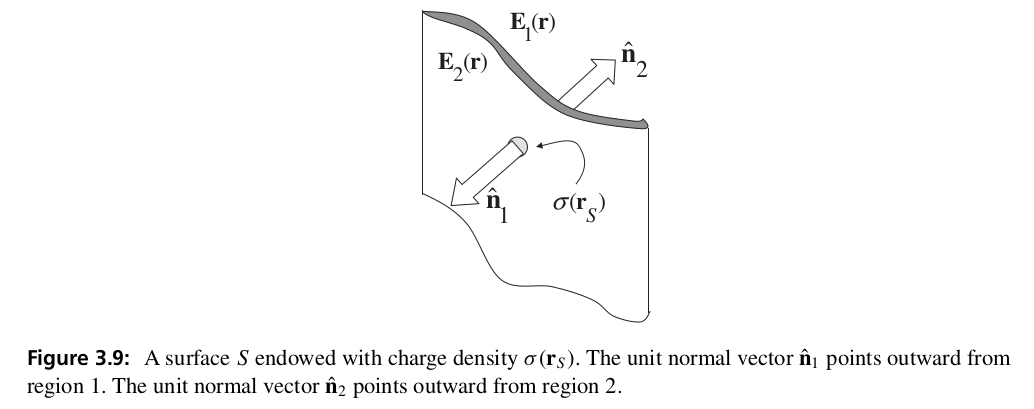
\includegraphics[width=0.6\textwidth]{3p9.png}
\end{center}

\begin{itemize}
\item Normais opostas em cada lado da superfície
\item Campo muda ao atravessar a superfície carregada
\end{itemize}

\end{frame}

%=================================================
\section{3.4.3 Força sobre uma superfície carregada}

%-------------------------------------------------
\begin{frame}{3.4.3 Força sobre a superfície}

\begin{mybox}{Problema - }
Como calcular a força sobre uma superfície carregada?
\end{mybox}

\begin{mybox}
Não é imediatamente óbvio como calcular a força de Coulomb sobre uma superfície carregada \(S\), pois (3.50) indica que \(\hat{\mathbf n}\cdot \mathbf E\) é descontínuo nesse ponto. Por outro lado, nenhum elemento de superfície pode exercer força sobre si mesmo. Portanto, a quantidade \(\mathbf E_S\) em (3.49) deve ser a única responsável pela força por unidade de área sentida em \(\mathbf r_S\). Como \(\hat{\mathbf n}_1 = -\hat{\mathbf n}_2\), a soma das duas equações em (3.49) fornece \(\mathbf E_S\) como a média simples de \(\mathbf E_1\) e \(\mathbf E_2\).
\end{mybox}


\begin{itemize}
\item Campo é descontínuo
\item Não podemos usar diretamente \(\mathbf E\)
\end{itemize}
\notas{15-16}
\end{frame}

%-------------------------------------------------
\begin{frame}{Campo efetivo}

\begin{mybox}{Ideia chave}
A força depende apenas do campo suave \(\mathbf E_S\).
\end{mybox}

\begin{eqbox}
\begin{equation}
\mathbf f = \sigma \mathbf E_S
= \frac{1}{2}\sigma(\mathbf E_1 + \mathbf E_2)
\tag{3.52}
\end{equation}
\end{eqbox}

\begin{alertblock}{Interpretação}
O campo relevante é a média dos dois lados.
\end{alertblock}

\end{frame}

%=================================================
\section{3.4.4 Solid Angle}

%-------------------------------------------------
\begin{frame}{3.4.4 Ângulo sólido}

\begin{mybox}{Definição: }
Ângulo sólido é a área projetada numa esfera unitária.
\end{mybox}

\begin{eqbox}
\begin{equation}
\Omega_S(\mathbf r)
=
\int_S d\mathbf S \cdot
\frac{\mathbf r_S - \mathbf r}{|\mathbf r_S - \mathbf r|^3}
\tag{3.53}
\end{equation}
\end{eqbox}
\notas{pag. 16-17}
\end{frame}

%-------------------------------------------------
\begin{frame}{Interpretação geométrica}

\begin{itemize}
\item Cada elemento \(dS\) projeta área na esfera unitária
\item Soma total define \(\Omega_S\)
\end{itemize}

\vspace{0.5cm}

\begin{center}
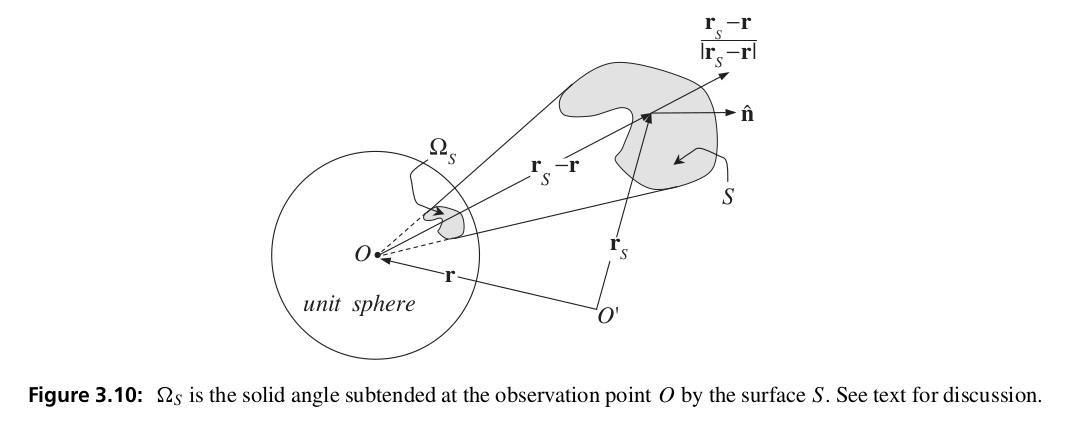
\includegraphics[width=0.6\textwidth]{3p10.png}
\end{center}

\end{frame}

%-------------------------------------------------
\begin{frame}{Elemento diferencial}

\begin{eqbox}
\begin{equation}
d\Omega_S = \frac{dS}{r_S^2}
= \sin\theta\, d\theta d\phi
\tag{3.54}
\end{equation}
\end{eqbox}

\end{frame}

%-------------------------------------------------
\begin{frame}{Resultado para superfície fechada}

\begin{eqbox}
\begin{equation}
\Omega_S =
\begin{cases}
4\pi & O \in V \\
0 & O \notin V
\end{cases}
\tag{3.55}
\end{equation}
\end{eqbox}

\begin{center}
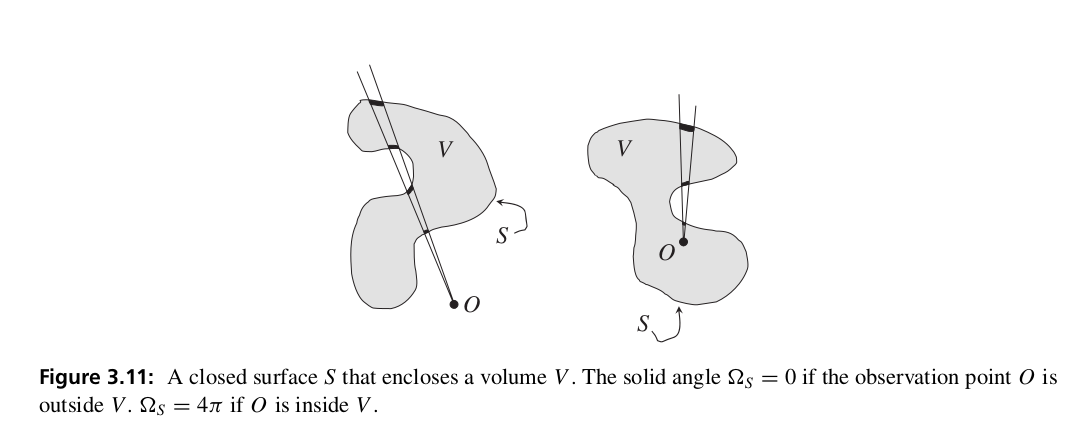
\includegraphics[width=0.6\textwidth]{3p11.png}
\end{center}

\end{frame}

%-------------------------------------------------
\begin{frame}{Lei de Gauss para carga pontual}

\begin{eqbox}
\begin{equation}
\Phi_E(S)
=
\int_S d\mathbf S \cdot \mathbf E
=
\frac{q}{4\pi\epsilon_0}\,\Omega_S
\tag{3.56}
\end{equation}
\end{eqbox}

\begin{alertblock}{Conclusão}
A Lei de Gauss surge naturalmente do ângulo sólido.
\end{alertblock}

\end{frame}

%=================================================
\section{Application 3.1}

%-------------------------------------------------
\begin{frame}{Linhas de campo: carga + campo uniforme}

\begin{mybox}{Situação}
Carga puntiforme em campo uniforme:
\[
\mathbf E = E \hat{\mathbf z}
\]
\end{mybox}

\vspace{0.4cm}

\begin{center}
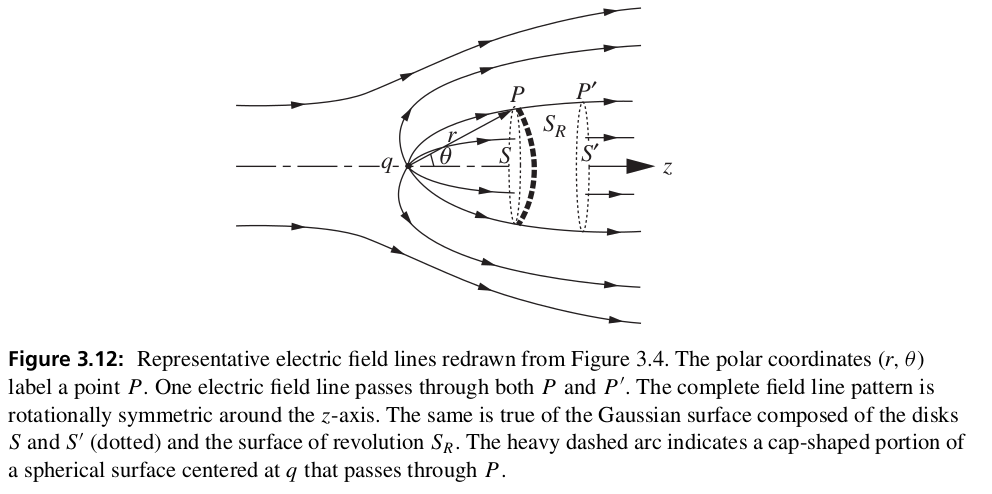
\includegraphics[width=0.6\textwidth]{3p12.png}
\end{center}

\end{frame}

%-------------------------------------------------
\begin{frame}{Fluxo total}

\begin{eqbox}
\begin{equation}
\Phi_E(S)
=
\frac{q}{4\pi\epsilon_0}\Omega_S + E\pi r^2 \sin^2\theta
\tag{3.57}
\end{equation}
\end{eqbox}

\end{frame}

%-------------------------------------------------
\begin{frame}{Ângulo sólido do disco}

\begin{eqbox}
\begin{equation}
\Omega_S
=
2\pi(1 - \cos\theta)
\tag{3.58}
\end{equation}
\end{eqbox}

\end{frame}

%-------------------------------------------------
\begin{frame}{Condição de fluxo}

\begin{eqbox}
\begin{equation}
\Phi_E(S') + \Phi_E(S) = 0
\tag{3.59}
\end{equation}
\end{eqbox}

\end{frame}

%-------------------------------------------------
\begin{frame}{Linhas de campo: carga + campo uniforme}

\begin{columns}[T,onlytextwidth]

%--------------------------------------
% Coluna da figura (reduzida)
%--------------------------------------
\column{0.45\textwidth}

\begin{block}{Visualização das linhas de campo}
\centering
\vspace{0.3cm}

\fbox{
\begin{minipage}[c][5.5cm][c]{0.8\linewidth}
\centering
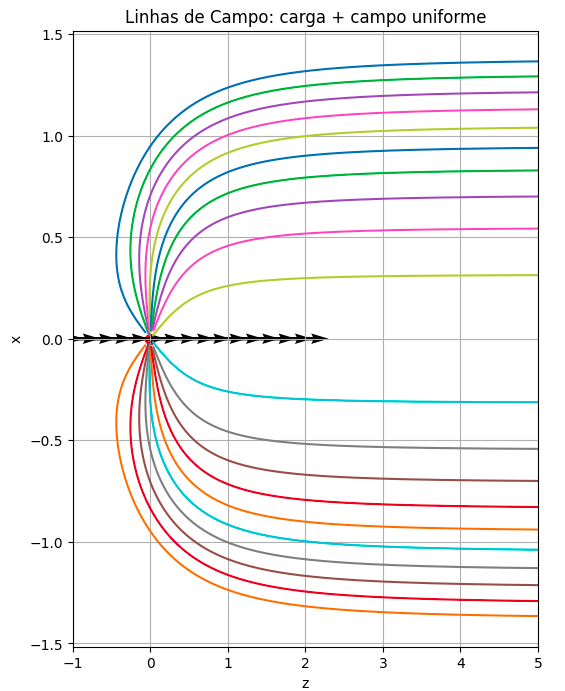
\includegraphics[width=0.8\linewidth]{cargaPLUSuniforme.png}
\end{minipage}
}

\vspace{0.3cm}
\end{block}

%--------------------------------------
% Coluna do texto/link (aumentada)
%--------------------------------------
\column{0.5\textwidth}

\begin{mybox}{Código no projeto Google Colab}
\small

\textbf{Acesse o código completo:}

\vspace{0.4cm}

\href{https://colab.research.google.com/drive/1ZlEup591atfG5S-tz5fw7LnFFov4j90c?usp=sharing}
{\textcolor{myblue}{\textbf{Abrir no Google Colab}}}

\vspace{0.6cm}

\begin{itemize}
\item Geração das linhas de campo
\item Controle do parâmetro $b$
\item Conversão para coordenadas cartesianas
\item Visualização gráfica completa
\end{itemize}

\end{mybox}

\end{columns}

\end{frame}

\begin{frame}{Exercício: linha infinita + campo uniforme}

\footnotesize

\begin{columns}[T,onlytextwidth]

%--------------------------------------
% Coluna esquerda
%--------------------------------------
\column{0.48\textwidth}

\begin{mybox}{Sistema}
Linha infinita (\(z\)) com densidade \(\lambda\), em
\[
\mathbf E_0 = E_0\,\hat{\mathbf x}.
\]
Plano \(xy\), coord. polares \((r,\phi)\).
\end{mybox}

\vspace{0.1cm}

\begin{block}{Analítico}
\begin{enumerate}
\item Campo da linha.
\item \(\mathbf E_0\) em \(\hat r,\hat\phi\).
\item Obter \(E_r, E_\phi\).

\end{enumerate}
\end{block}

%--------------------------------------
% Coluna direita
%--------------------------------------
\column{0.48\textwidth}

\begin{block}{Linhas}
\begin{enumerate}
\setcounter{enumi}{4}
\item Encontrar:
\[
F(r,\phi)=C.
\]
\end{enumerate}
\end{block}

\vspace{0.1cm}

\begin{alertblock}{Código}
\begin{itemize}
\item plotar para vários \(C\);
\item fazer 3 plots com diferentes \(\lambda/E_0\). Que padrão você percebe?
\end{itemize}
\end{alertblock}

\vspace{0.1cm}

\begin{mybox}{Discussão}
\begin{itemize}
\item perto da linha;
\item longe;
\item efeito de \(\lambda/E_0\).
\end{itemize}
\end{mybox}

\end{columns}

\end{frame}
%=================================================
\section{3.5 Energia Potencial Eletrostática}

%-------------------------------------------------
\begin{frame}{3.5 Energia Potencial: ideia física}

\begin{mybox}{Ponto de partida}
Em mecânica, a energia potencial mede o trabalho que a força pode realizar.
Se uma força desloca uma partícula por \(\delta \mathbf{s}\), a variação da energia potencial é:
\end{mybox}

\begin{eqbox}
\begin{equation}
\delta V = -\mathbf F \cdot \delta \mathbf s
\tag{3.61}
\end{equation}
\end{eqbox}

\begin{alertblock}{Comentário físico}
O sinal negativo significa que, se a força realiza trabalho positivo, a energia potencial diminui.
\end{alertblock}

\end{frame}


%-------------------------------------------------
\begin{frame}{Força como gradiente da energia}

\begin{mybox}{Da forma diferencial para a forma local}
Como
\[
\delta V = \nabla V \cdot \delta \mathbf{s},
\]
comparando com
\[
\delta V = -\mathbf F \cdot \delta \mathbf{s},
\]
obtemos:
\end{mybox}

\begin{eqbox}
\begin{equation}
\mathbf F = -\nabla V
\tag{3.62}
\end{equation}
\end{eqbox}

\begin{alertblock}{Interpretação}
A força aponta para a direção em que a energia potencial diminui mais rapidamente.
\end{alertblock}

\end{frame}

%-------------------------------------------------
\begin{frame}{Energia potencial elétrica de uma carga}

\begin{mybox}{Força elétrica sobre uma carga: }
Para uma carga \(q\) em um campo elétrico:
\[
\mathbf F = q\mathbf E.
\]
Na eletrostática, o campo pode ser escrito em termos do potencial:
\[
\mathbf E = -\nabla \varphi.
\]
\end{mybox}

\begin{eqbox}
\begin{equation}
\mathbf F
=
q\mathbf E
=
-q\nabla\varphi
=
-\nabla(q\varphi)
\end{equation}
\end{eqbox}

\end{frame}

%-------------------------------------------------
\begin{frame}{Energia potencial elétrica}

\begin{mybox}{Comparando com \(\mathbf F=-\nabla V\)}
Como
\[
\mathbf F = -\nabla(q\varphi),
\]
identificamos a energia potencial elétrica:
\end{mybox}

\begin{eqbox}
\begin{equation}
V_E = q\,\varphi(\mathbf r)
\tag{3.63}
\end{equation}
\end{eqbox}

\begin{alertblock}{Comentário}
O potencial elétrico \(\varphi\) é energia potencial por unidade de carga.
\[
\varphi = \frac{V_E}{q}.
\]
\end{alertblock}

\end{frame}

%-------------------------------------------------
\begin{frame}{De uma carga para uma distribuição}

\begin{mybox}{Ideia de superposição: }
Uma distribuição contínua de carga pode ser pensada como muitos elementos infinitesimais:
\[
dq = \rho_2(\mathbf r)\,d^3r.
\]
Cada elemento possui energia:
\[
dV_E = dq\,\varphi_1(\mathbf r).
\]
\end{mybox}

\begin{eqbox}
\begin{equation}
dV_E
=
\rho_2(\mathbf r)\,\varphi_1(\mathbf r)\,d^3r
\end{equation}
\end{eqbox}

\end{frame}

%-------------------------------------------------
\begin{frame}{Energia de uma distribuição em um campo externo}

\begin{mybox}{Somando todos os elementos: }
Integrando sobre toda a distribuição \(\rho_2\), obtemos:
\end{mybox}

\begin{eqbox}
\begin{equation}
V_E = \int d^3r\, \rho_2(\mathbf r)\,\varphi_1(\mathbf r)
\tag{3.64}
\end{equation}
\end{eqbox}

\begin{alertblock}{Cuidado conceitual}
Aqui \(\varphi_1\) é o potencial produzido por outra distribuição, \(\rho_1\).
Portanto, esta é a energia de \(\rho_2\) colocada no campo de \(\rho_1\).
\end{alertblock}

\end{frame}

%=================================================
\section{3.5.1 Força via variação da energia}

%-------------------------------------------------
\begin{frame}{3.5.1 Como extrair a força da energia?}

\begin{mybox}{Estratégia: }
Vamos deslocar rigidamente a distribuição \(\rho_2\) por um pequeno vetor \(\delta\mathbf{s}\).
\end{mybox}

\begin{center}
\begin{tikzpicture}[scale=0.9]

% distribuição inicial
\draw[fill=mycyan!20, draw=myblue, thick] (0,0) ellipse (1.1 and 0.6);
\node at (0,0) {\(\rho_2\)};

% distribuição deslocada
\draw[fill=mycyan!10, draw=myblue, dashed, thick] (4,0) ellipse (1.1 and 0.6);
\node at (4,0) {\(\rho_2'\)};

% vetor deslocamento conectando centros
\draw[->, thick, myred] (0,0) -- (4,0);
\node[above] at (2,0) {\(\delta\mathbf{s}\)};

\end{tikzpicture}
\end{center}

\begin{alertblock}{Ideia física}
Se a energia muda quando deslocamos a distribuição, essa variação revela a força resultante sobre ela.
\end{alertblock}

\end{frame}

%-------------------------------------------------
\begin{frame}{Como a densidade muda sob deslocamento}

\begin{columns}[T,onlytextwidth]

%--------------------------------------
% Coluna da figura
%--------------------------------------
\column{0.45\textwidth}

\begin{center}
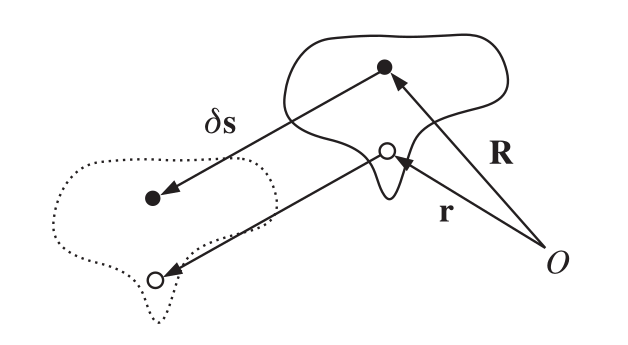
\includegraphics[width=\linewidth]{3p13.png}
\end{center}

%--------------------------------------
% Coluna do conteúdo
%--------------------------------------
\column{0.55\textwidth}

\begin{mybox}{Distribuição deslocada}
Após deslocar a distribuição por \(\delta\mathbf{s}\), a nova densidade no ponto \(\mathbf r\) é:
\[
\rho_2(\mathbf r-\delta\mathbf{s}).
\]
\end{mybox}

\begin{eqbox}
\begin{equation}
\delta \rho_2(\mathbf r)
=
\rho_2(\mathbf r-\delta \mathbf s) - \rho_2(\mathbf r)
\tag{3.65}
\end{equation}
\end{eqbox}

\begin{alertblock}{Interpretação}
A carga que agora está em \(\mathbf R + \delta s\) veio de uma posição ligeiramente anterior, deslocada de \(\delta\mathbf{R}\).
\end{alertblock}

\end{columns}

\end{frame}

%-------------------------------------------------
\begin{frame}{Expansão de Taylor da densidade}

\begin{mybox}{Para deslocamentos pequenos: }
Expandimos em primeira ordem:
\[
\rho_2(\mathbf r-\delta\mathbf{s})
\simeq
\rho_2(\mathbf r)
-
\delta\mathbf{s}\cdot\nabla\rho_2(\mathbf r).
\]
\end{mybox}

\begin{eqbox}
\begin{equation}
\delta \rho_2(\mathbf r)
\simeq
-\delta\mathbf{s}\cdot\nabla\rho_2(\mathbf r)
\end{equation}
\end{eqbox}

\begin{alertblock}{Comentário}
A densidade muda apenas onde há variação espacial de \(\rho_2\).
Se \(\rho_2\) fosse perfeitamente uniforme em todo o espaço, esse termo seria nulo.
\end{alertblock}

\end{frame}

%-------------------------------------------------
\begin{frame}{Variação da energia}

\begin{mybox}{Energia antes e depois do deslocamento}
Como
\[
V_E = \int d^3r\,\rho_2(\mathbf r)\varphi_1(\mathbf r),
\]
a variação da energia é:
\end{mybox}

\begin{eqbox}
\begin{equation}
\delta V_E
=
\int d^3r\,\varphi_1(\mathbf r)\,\delta\rho_2(\mathbf r)
\tag{3.66}
\end{equation}
\end{eqbox}

\begin{alertblock}{Ponto importante: }
O potencial \(\varphi_1\) fica fixo; quem está sendo deslocada é a distribuição \(\rho_2\).
\end{alertblock}

\end{frame}

%-------------------------------------------------
\begin{frame}{Substituindo a expansão de Taylor}

\begin{mybox}{Usando}
\[
\delta\rho_2
\simeq
-\delta\mathbf{s}\cdot\nabla\rho_2,
\]
temos:
\end{mybox}

\begin{eqbox}
\begin{equation}
\delta V_E
=
-\int d^3r\,
\varphi_1(\mathbf r)
\,
\delta\mathbf{s}\cdot\nabla\rho_2(\mathbf r)
\tag{3.67}
\end{equation}
\end{eqbox}

\begin{alertblock}{Leitura física}
A mudança de energia depende de como a distribuição de carga ``atravessa'' regiões de potencial diferente.
\end{alertblock}

\end{frame}

%-------------------------------------------------
\begin{frame}{Preparando a integração por partes}

\begin{mybox}{Como \(\delta\mathbf{s}\) é constante}
Podemos escrever:
\[
\delta\mathbf{s}\cdot\nabla\rho_2
=
\nabla\rho_2\cdot\delta\mathbf{s}.
\]
Assim,
\[
\delta V_E
=
-\delta\mathbf{s}\cdot
\int d^3r\,\varphi_1\nabla\rho_2.
\]
\end{mybox}

\begin{alertblock}{Objetivo}
Queremos trocar a derivada de \(\rho_2\) para \(\varphi_1\), pois \(\nabla\varphi_1\) está ligado ao campo elétrico.
\end{alertblock}

\end{frame}

%-------------------------------------------------
\begin{frame}{Integração por partes}

\begin{mybox}{Identidade usada - }
Para funções que desaparecem suficientemente longe:
\[
\int d^3r\,\varphi_1\nabla\rho_2
=
-\int d^3r\,\rho_2\nabla\varphi_1.
\]
\end{mybox}

\begin{eqbox}
\begin{equation}
\delta V_E
=
\int d^3r\,
\rho_2(\mathbf r)
\nabla\varphi_1(\mathbf r)\cdot\delta\mathbf{s}
\tag{3.68}
\end{equation}
\end{eqbox}

\begin{alertblock}{Funções de Suporte Compacto}
O termo de superfície é descartado porque a distribuição é localizada ou porque os campos decaem no infinito.
\end{alertblock}

\end{frame}

%-------------------------------------------------
\begin{frame}{Aparece o campo elétrico}

\begin{mybox}{Usando}
\[
\mathbf E_1 = -\nabla\varphi_1,
\]
a variação da energia fica:
\[
\delta V_E
=
-\int d^3r\,
\rho_2(\mathbf r)\mathbf E_1(\mathbf r)\cdot\delta\mathbf{s}.
\]
\end{mybox}

\begin{eqbox}
\begin{equation}
\delta V_E
=
-\mathbf F\cdot\delta\mathbf{s}
\end{equation}
\end{eqbox}

\begin{alertblock}{Comparação}
Comparando as duas expressões, identificamos a força total sobre \(\rho_2\).
\end{alertblock}

\end{frame}

%-------------------------------------------------
\begin{frame}{Resultado: força sobre uma distribuição}

\begin{eqbox}
\begin{equation}
\mathbf F
=
-\frac{\partial V_E}{\partial \mathbf s}
=
\int d^3r\, \rho_2(\mathbf r)\,\mathbf E_1(\mathbf r)
\tag{3.69}
\end{equation}
\end{eqbox}

\begin{mybox}{Interpretação}
Cada elemento de carga \(dq=\rho_2d^3r\) sofre uma força:
\[
d\mathbf F = dq\,\mathbf E_1.
\]
Somando todos os elementos:
\[
\mathbf F = \int d\mathbf F.
\]
\end{mybox}

\begin{alertblock}{Conclusão}
A derivação por energia reproduz exatamente a soma das forças de Coulomb.
\end{alertblock}

\end{frame}

%=================================================
\section{3.5.2 Relação de reciprocidade de Green}

%-------------------------------------------------
\begin{frame}{3.5.2 Relação de reciprocidade de Green}

\begin{mybox}{Duas distribuições: }
Considere duas distribuições:
\[
\rho_1 \longrightarrow \varphi_1,
\qquad
\rho_2 \longrightarrow \varphi_2.
\]
A energia de \(\rho_2\) no potencial de \(\rho_1\) é:
\[
V_E=\int d^3r\,\rho_2\varphi_1.
\]
\end{mybox}

\begin{alertblock}{Pergunta}
Essa energia muda se trocarmos os papéis de fonte e carga-teste?
\end{alertblock}

\end{frame}

%-------------------------------------------------
\begin{frame}{Reciprocidade: resultado}

\begin{eqbox}
\begin{equation}
\int d^3r\, \rho_1(\mathbf r)\varphi_2(\mathbf r)
=
\int d^3r\, \rho_2(\mathbf r)\varphi_1(\mathbf r)
\tag{3.70}
\end{equation}
\end{eqbox}

\begin{alertblock}{Significado físico}
A energia de interação entre duas distribuições é simétrica:
não importa se dizemos que \(\rho_1\) está no potencial de \(\rho_2\)
ou que \(\rho_2\) está no potencial de \(\rho_1\).
\end{alertblock}

\end{frame}

%-------------------------------------------------
\begin{frame}{Por que a reciprocidade é útil?}

\begin{mybox}{Liberdade de escolha: }
A mesma energia pode ser escrita como:
\[
V_E
=
\int d^3r\,\rho_2\varphi_1
=
\int d^3r\,\rho_1\varphi_2.
\]
\end{mybox}

\begin{eqbox}
\begin{equation}
V_E
=
\int d^3r\, \rho_1(\mathbf r)\varphi_2(\mathbf r)
\tag{3.71}
\end{equation}
\end{eqbox}

\begin{alertblock}{Comentário}
Escolhemos a forma mais simples para o problema.
Às vezes é mais fácil integrar sobre \(\rho_1\); em outros casos, sobre \(\rho_2\).
\end{alertblock}

\end{frame}

%-------------------------------------------------
\begin{frame}{Duas distribuições esféricas não sobrepostas}

\begin{columns}[T,onlytextwidth]

\column{0.48\textwidth}

\begin{mybox}{Ideia}
Para uma distribuição esférica, o potencial externo é igual ao de uma carga puntiforme no centro:
\[
\varphi(r)=\frac{Q}{4\pi\epsilon_0 r}.
\]
\end{mybox}

\begin{alertblock}{Condição}
As distribuições não podem se sobrepor.
\end{alertblock}

\column{0.48\textwidth}

\begin{center}
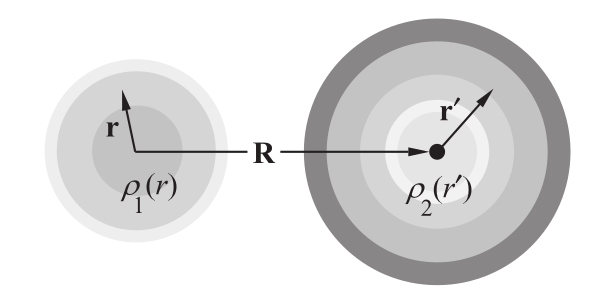
\includegraphics[width=0.9\textwidth]{3p14.png}
\end{center}

\end{columns}

\end{frame}

%-------------------------------------------------
\begin{frame}{Energia entre duas distribuições esféricas}

\begin{mybox}{Usando reciprocidade}
Podemos tratar cada distribuição esférica, externamente, como se toda a carga estivesse concentrada no centro.
\end{mybox}

\begin{eqbox}
\begin{equation}
V_E = \frac{Q_1 Q_2}{4\pi\epsilon_0 R}
\tag{3.72}
\end{equation}
\end{eqbox}

\begin{alertblock}{Resultado}
A energia de interação entre duas distribuições esféricas não sobrepostas é a mesma de duas cargas puntiformes separadas por \(R\).
\end{alertblock}

\end{frame}

%=================================================
\section{Exemplo 3.5}

%-------------------------------------------------
\begin{frame}{Exemplo 3.5}

\begin{mybox}{
Use a relação de reciprocidade de Green e uma esfera oca com carga distribuída uniformemente sobre sua superfície para provar o seguinte ``teorema do valor médio'': a média de $\varphi(\mathbf r)$ sobre uma superfície esférica $S$ que envolve uma região livre de cargas é igual ao potencial no centro da esfera:
}
\end{mybox}

\begin{eqbox}
\begin{equation}
\frac{1}{4\pi R^2} \int_{S} dS\, \varphi(\mathbf r) = \varphi(0).
\tag{3.5}
\end{equation}
\end{eqbox}
\notas{pag 21-23}
\end{frame}

%-------------------------------------------------
\begin{frame}{Estratégia da prova}

\begin{columns}[T,onlytextwidth]

\column{0.52\textwidth}

\begin{mybox}{Truque:}
Usamos a reciprocidade de Green com um sistema auxiliar simples:
uma casca esférica uniformemente carregada.
\end{mybox}

\begin{itemize}
\item A casca gera potencial constante em seu interior.
\item A distribuição externa gera o potencial \(\varphi\).
\item A reciprocidade liga os dois pontos de vista.
\end{itemize}

\column{0.44\textwidth}

\begin{center}
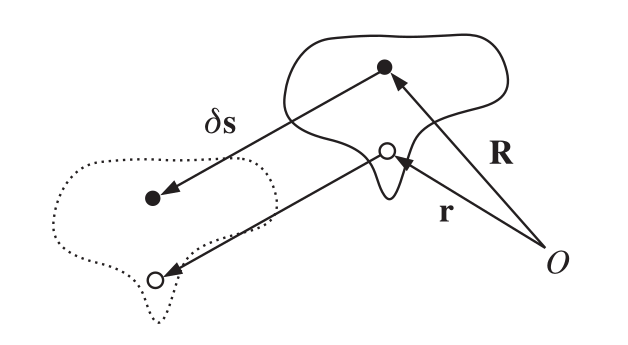
\includegraphics[width=0.95\textwidth]{3p13.png}
\end{center}

\end{columns}

\end{frame}

%-------------------------------------------------
\begin{frame}{Sistema auxiliar: casca esférica}

\begin{mybox}{Escolha auxiliar}
Considere uma casca esférica de raio \(R\), carga total \(Q\), e densidade superficial uniforme:
\[
\sigma = \frac{Q}{4\pi R^2}.
\]
\end{mybox}

\begin{eqbox}
\begin{equation}
\rho_{\rm casca}(\mathbf r)
=
\sigma\,\delta(r-R)
\end{equation}
\end{eqbox}

\begin{alertblock}{Por que essa escolha é útil?}
Porque o potencial produzido pela casca é constante em qualquer ponto dentro dela.
\end{alertblock}

\end{frame}

%-------------------------------------------------
\begin{frame}{Potencial da casca no interior}

\begin{mybox}{Resultado conhecido}
Para qualquer ponto dentro da casca:
\[
\varphi_{\rm casca}
=
\frac{Q}{4\pi\epsilon_0 R}.
\]
\end{mybox}

\begin{alertblock}{Comentário}
Esse potencial é o mesmo no centro e em qualquer outro ponto interno.
Isso é o que torna a casca um sistema auxiliar poderoso.
\end{alertblock}

\end{frame}

%-------------------------------------------------
\begin{frame}{Aplicando reciprocidade}

\begin{mybox}{Reciprocidade}
Tomamos:
\[
\rho_1 = \rho_{\rm externa},
\qquad
\rho_2 = \rho_{\rm casca}.
\]
Então:
\[
\int d^3r\,\rho_{\rm externa}\varphi_{\rm casca}
=
\int d^3r\,\rho_{\rm casca}\varphi.
\]
\end{mybox}

\begin{alertblock}{Ideia}
O lado esquerdo usa o potencial simples da casca.
O lado direito vira uma média do potencial \(\varphi\) sobre a superfície.
\end{alertblock}

\end{frame}

%-------------------------------------------------
\begin{frame}{Lado esquerdo da reciprocidade}

\begin{mybox}{Como \(\varphi_{\rm casca}\) é constante na região interna}
\[
\varphi_{\rm casca}
=
\frac{Q}{4\pi\epsilon_0 R}.
\]
Logo:
\[
\int d^3r\,\rho_{\rm externa}\varphi_{\rm casca}
=
\frac{Q}{4\pi\epsilon_0 R}
\int d^3r\,\rho_{\rm externa}.
\]
\end{mybox}

\begin{alertblock}{Interpretação}
Esse lado representa a energia da distribuição externa no potencial constante da casca.
\end{alertblock}

\end{frame}

%-------------------------------------------------
\begin{frame}{Lado direito da reciprocidade}

\begin{mybox}{A carga está apenas na superfície}
Como a casca possui densidade superficial uniforme:
\[
dq = \sigma\,dS.
\]
Então:
\[
\int d^3r\,\rho_{\rm casca}\varphi
=
\int_S \sigma\,\varphi\,dS.
\]
\end{mybox}

\begin{eqbox}
\begin{equation}
\int d^3r\,\rho_{\rm casca}\varphi
=
\frac{Q}{4\pi R^2}\int_S \varphi\,dS
\end{equation}
\end{eqbox}

\end{frame}

%-------------------------------------------------
\begin{frame}{Obtendo o valor médio}

\begin{mybox}{Usando reciprocidade}
A igualdade entre os dois lados leva a:
\[
\frac{Q}{4\pi R^2}\int_S \varphi\,dS
=
Q\,\varphi(0).
\]
Cancelando \(Q\):
\end{mybox}

\begin{eqbox}
\begin{equation}
\frac{1}{4\pi R^2}\int_S dS\,\varphi(\mathbf r)
=
\varphi(0)
\end{equation}
\end{eqbox}

\begin{alertblock}{Conclusão}
O potencial no centro é a média do potencial sobre a superfície.
\end{alertblock}

\end{frame}

%-------------------------------------------------
\begin{frame}{Mensagem física do exemplo}

\begin{alertblock}{Conclusão principal}
Em regiões sem carga, o potencial eletrostático é uma função harmônica:
\[
\nabla^2\varphi = 0.
\]
Funções harmônicas obedecem ao teorema do valor médio.
\end{alertblock}

\begin{mybox}{Consequência importante}
O potencial não pode ter máximos ou mínimos locais em uma região vazia de cargas.
Isso está por trás de muitos resultados de estabilidade em eletrostática.
\end{mybox}

\end{frame}




\section{Energia Eletrostática Total}

%-------------------------------------------------
\begin{frame}{3.6 Energia Eletrostática Total}

\begin{mybox}{Definição: }
A energia eletrostática total $U_E$ é definida como o trabalho total necessário para montar uma distribuição de cargas a partir de um estado inicial em que toda a carga está dispersa no infinito.
\end{mybox}

\begin{itemize}
\item O processo é realizado quase-estaticamente
\item Não há dissipação de energia
\item O processo é reversível (termodinamicamente)
\end{itemize}

\end{frame}

%-------------------------------------------------
\begin{frame}{Interpretação Física}

\begin{itemize}
\item $U_E$ atinge valor mínimo no estado fundamental
\item Pode depender de parâmetros variacionais
\item Minimizar $U_E$ $\Rightarrow$ aproximação do estado fundamental
\end{itemize}

\end{frame}

%-------------------------------------------------
\begin{frame}{Sistema de Cargas Puntiformes}

\begin{mybox}{Configuração: }
Considere $N$ cargas puntiformes $q_k$ nas posições $\mathbf r_k$.
\end{mybox}

\begin{itemize}
\item Primeira carga: não exige trabalho ($E=0$)
\item Segunda carga: trabalho contra a força de Coulomb
\end{itemize}

\begin{eqbox}
\begin{equation}
W_{12}
=
q_2 \varphi_1(r_2)
=
\frac{1}{4\pi\epsilon_0}
\frac{q_1 q_2}{|\mathbf r_1 - \mathbf r_2|}
\tag{3.73}
\end{equation}
\end{eqbox}

\end{frame}

%-------------------------------------------------
\begin{frame}{Generalização para $N$ Cargas}

\begin{mybox}{Energia Total}
Somando todas as interações:
\end{mybox}

\begin{eqbox}
\begin{equation}
U_E
=
\frac{1}{4\pi\epsilon_0}
\sum_{j=1}^{N}
\sum_{i>j}^{N}
\frac{q_i q_j}{|\mathbf r_i - \mathbf r_j|}
\tag{3.74}
\end{equation}
\end{eqbox}

\end{frame}

%-------------------------------------------------
\begin{frame}{Forma Alternativa}

\begin{alertblock}{Correção de Supercontagem}
Cada par é contado duas vezes na soma dupla.
\end{alertblock}

\begin{eqbox}
\begin{equation}
U_E
=
\frac{1}{2}
\sum_{i=1}^{N}
q_i \varphi(\mathbf r_i)
\tag{3.75}
\end{equation}
\end{eqbox}

\end{frame}

%-------------------------------------------------
\begin{frame}{Distribuição Contínua}

\begin{mybox}{Limite Contínuo}
Substituímos somas por integrais:
\end{mybox}

\begin{eqbox}
\begin{equation}
U_E
=
\frac{1}{8\pi\epsilon_0}
\int d^3r
\int d^3r'
\frac{\rho(\mathbf r)\rho(\mathbf r')}{|\mathbf r - \mathbf r'|}
\tag{3.76}
\end{equation}
\end{eqbox}

\begin{eqbox}
\begin{equation}
U_E
=
\frac{1}{2}
\int d^3r\, \rho(\mathbf r)\varphi(\mathbf r)
\tag{3.76}
\end{equation}
\end{eqbox}

\end{frame}

%-------------------------------------------------
\begin{frame}{Exemplo: Esfera Uniforme}

\begin{mybox}{Construção: }
Montamos a esfera adicionando camadas esféricas de espessura $dr$.
\end{mybox}

\begin{itemize}
\item Densidade: $\rho = \frac{Q}{\frac{4}{3}\pi R^3}$
\item Incremento de carga: $dq = 4\pi r^2 \rho\, dr$
\end{itemize}

\end{frame}

%-------------------------------------------------
\begin{frame}{Energia da Esfera: ideia da construção}

\begin{mybox}{Montagem por camadas: }
Construímos uma esfera uniformemente carregada adicionando cascas esféricas infinitesimais de raio $r$ e espessura $dr$.
\end{mybox}

\begin{eqbox}
\begin{equation}
dq = 4\pi r^2 \rho\, dr .
\label{eq:dq_camada}
\end{equation}
\end{eqbox}

\begin{mybox}{Carga já montada até o raio $r$}
\begin{equation}
q(r)=\frac{4\pi}{3}r^3\rho .
\label{eq:carga_interna_r}
\end{equation}
\end{mybox}

\end{frame}

%-------------------------------------------------
\begin{frame}{Energia da Esfera: trabalho infinitesimal}

\begin{mybox}{Potencial na superfície da esfera parcial: }
No instante em que a esfera tem raio $r$, o potencial em sua superfície é
\end{mybox}

\begin{eqbox}
\begin{equation}
\varphi_s(r)
=
\frac{1}{4\pi\epsilon_0}\frac{q(r)}{r}
=
\frac{1}{4\pi\epsilon_0}
\frac{\frac{4\pi}{3}r^3\rho}{r}
=
\frac{\rho r^2}{3\epsilon_0}.
\label{eq:potencial_superficie_esfera}
\end{equation}
\end{eqbox}

\begin{mybox}{Trabalho para trazer a próxima camada}
\begin{equation}
dU_E = \varphi_s(r)\,dq .
\label{eq:dU_phi_dq}
\end{equation}
\end{mybox}

\end{frame}

%-------------------------------------------------
\begin{frame}{Energia da Esfera: integração}

Substituindo \eqref{eq:dq_camada} e \eqref{eq:potencial_superficie_esfera} em \eqref{eq:dU_phi_dq}:

\begin{eqbox}
\begin{align}
dU_E
&=
\left(\frac{\rho r^2}{3\epsilon_0}\right)
\left(4\pi r^2\rho\,dr\right)
\nonumber\\
&=
\frac{4\pi}{3\epsilon_0}\rho^2 r^4\,dr .
\label{eq:dU_esfera}
\end{align}
\end{eqbox}

Logo,

\begin{eqbox}
\begin{equation}
U_E
=
\frac{4\pi}{3\epsilon_0}
\rho^2
\int_0^R r^4\,dr .
\label{eq:UE_integral_esfera}
\end{equation}
\end{eqbox}

\end{frame}

%-------------------------------------------------
\begin{frame}{Energia da Esfera: resultado final}

A integral radial é

\begin{equation}
\int_0^R r^4\,dr = \frac{R^5}{5}.
\label{eq:int_r4}
\end{equation}

Portanto,

\begin{eqbox}
\begin{equation}
U_E
=
\frac{4\pi}{15\epsilon_0}\rho^2 R^5 .
\label{eq:UE_rho_R}
\end{equation}
\end{eqbox}

Como

\begin{equation}
Q=\frac{4\pi}{3}R^3\rho
\quad\Rightarrow\quad
\rho=\frac{3Q}{4\pi R^3},
\label{eq:rho_QR}
\end{equation}

\end{frame}

\begin{frame}

obtemos

\begin{eqbox}
\begin{equation}
U_E
=
\frac{3}{5}
\frac{Q^2}{4\pi\epsilon_0 R}.
\tag{3.77}
\end{equation}
\end{eqbox}

\end{frame}

%-------------------------------------------------
\begin{frame}{Construção Contínua: ideia}

\begin{mybox}{Método alternativo}
Em vez de montar uma esfera camada por camada, podemos montar uma distribuição qualquer aumentando sua densidade gradualmente:
\end{mybox}

\begin{eqbox}
\begin{equation}
\rho_\lambda(\mathbf r)=\lambda \rho(\mathbf r),
\qquad 0\leq \lambda \leq 1 .
\label{eq:rho_lambda}
\end{equation}
\end{eqbox}

Por linearidade da equação de Poisson,

\begin{eqbox}
\begin{equation}
\varphi_\lambda(\mathbf r)=\lambda \varphi(\mathbf r).
\label{eq:phi_lambda}
\end{equation}
\end{eqbox}

\end{frame}

%-------------------------------------------------
\begin{frame}{Construção Contínua: trabalho infinitesimal}

Ao aumentar o parâmetro de $\lambda$ para $\lambda+d\lambda$, a densidade adicionada é

\begin{eqbox}
\begin{equation}
d\rho(\mathbf r)=d\lambda\,\rho(\mathbf r).
\label{eq:drho_lambda}
\end{equation}
\end{eqbox}

O trabalho infinitesimal para adicionar essa carga ao potencial já existente é

\begin{eqbox}
\begin{align}
dU_E
&=
\int d^3r\, d\rho(\mathbf r)\,\varphi_\lambda(\mathbf r)
\nonumber\\
&=
\int d^3r\,
\left[d\lambda\,\rho(\mathbf r)\right]
\left[\lambda\varphi(\mathbf r)\right]
\nonumber\\
&=
\lambda\,d\lambda
\int d^3r\,\rho(\mathbf r)\varphi(\mathbf r).
\label{eq:dU_lambda}
\end{align}
\end{eqbox}

\end{frame}

%-------------------------------------------------
\begin{frame}{Construção Contínua: resultado geral}

Integrando de $\lambda=0$ até $\lambda=1$:

\begin{eqbox}
\begin{align}
U_E
&=
\int_0^1
\lambda\,d\lambda
\int d^3r\,\rho(\mathbf r)\varphi(\mathbf r)
\nonumber\\
&=
\left(\int_0^1 \lambda\,d\lambda\right)
\int d^3r\,\rho(\mathbf r)\varphi(\mathbf r)
\nonumber\\
&=
\frac{1}{2}
\int d^3r\,\rho(\mathbf r)\varphi(\mathbf r).
\tag{3.78}
\end{align}
\end{eqbox}

\begin{alertblock}{Origem do fator $1/2$}
Ele aparece porque o potencial não está pronto desde o início, ele cresce junto com a carga durante a montagem da distribuição. Logo vem de uma média.
\end{alertblock}

\end{frame}

%-------------------------------------------------
\begin{frame}{Observação Importante: divergência}

\begin{alertblock}{Carga puntiforme}
Para uma carga puntiforme, a energia eletrostática própria diverge.
\end{alertblock}

Pela energia da esfera uniformemente carregada,

\begin{eqbox}
\begin{equation}
U_E
=
\frac{3}{5}
\frac{Q^2}{4\pi\epsilon_0 R}.
\label{eq:UE_divergencia}
\end{equation}
\end{eqbox}

No limite de carga puntiforme,

\begin{eqbox}
\begin{equation}
R\to 0
\qquad\Rightarrow\qquad
U_E\to \infty .
\label{eq:limite_divergencia}
\end{equation}
\end{eqbox}

\begin{mybox}{Interpretação}
Essa divergência reflete uma limitação fundamental da eletrodinâmica clássica quando cargas puntiformes são tratadas literalmente.
\end{mybox}

\end{frame}




\begin{frame}{Exercício 3.15}

\begin{mybox}{
Considere que o espaço entre duas esferas concêntricas de raios $a$ e $R \geq a$ esteja preenchido uniformemente com carga.
}
\end{mybox}

\begin{itemize}
\item[(a)] Calcule a energia total $U_E$ em termos da carga total $Q$ e da variável $x = a/R$. Verifique os limites $a = 0$ e $a = R$.

\vspace{0.3cm}

\item[(b)] Minimize $U_E$ em relação a $x$ (mantendo a carga total $Q$ constante). Identifique o sistema físico que realiza o mínimo encontrado.
\end{itemize}
\notas{pag: 24-30}
\end{frame}


%-------------------------------------------------
\begin{frame}{Força sobre uma distribuição de carga}

\begin{mybox}
Campo elétrico gerado por $\rho(\mathbf r)$:
\[
\mathbf E(\mathbf r)
\]
\end{mybox}

\begin{eqbox}
\begin{equation}
\mathbf F = \int_V d^3r\, \rho(\mathbf r)\,\mathbf E(\mathbf r)
\label{eq:3.90}
\end{equation}
\end{eqbox}

\begin{itemize}
\item Força total = soma da força local $\rho \mathbf E$
\item Objetivo: eliminar $\rho$
\end{itemize}
\notas{pag 31-38}
\end{frame}

%-------------------------------------------------
\begin{frame}{Usando a Lei de Gauss}

\begin{eqbox}
\begin{equation}
\nabla \cdot \mathbf E = \frac{\rho}{\epsilon_0}
\end{equation}
\end{eqbox}

Substituindo em (\ref{eq:3.90}):

\begin{eqbox}
\begin{equation}
F_i = \epsilon_0 \int_V d^3r\, (\nabla \cdot \mathbf E)\, E_i
\end{equation}
\end{eqbox}

\begin{mybox}
Usando notação de índices:
\[
\nabla \cdot \mathbf E = \partial_j E_j
\]
\end{mybox}

\end{frame}

%-------------------------------------------------
\begin{frame}{Manipulação vetorial (passo chave)}

\begin{eqbox}
\begin{equation}
F_i = \epsilon_0 \int_V d^3r\, (\partial_j E_j)\, E_i
\end{equation}
\end{eqbox}

Somamos e subtraímos um termo:

\begin{eqbox}
\begin{equation}
F_i = \epsilon_0 \int_V d^3r
\left[
\partial_j (E_j E_i) - E_j \partial_j E_i
\right]
\end{equation}
\end{eqbox}

\begin{mybox}
Identidade usada:
\[
\partial_j (E_j E_i) = (\partial_j E_j)E_i + E_j(\partial_j E_i)
\]
\end{mybox}

\end{frame}

%-------------------------------------------------
\begin{frame}{Uso de $\nabla \times \mathbf E = 0$}

\begin{mybox}
Campo eletrostático:
\[
\nabla \times \mathbf E = 0
\Rightarrow \partial_j E_i = \partial_i E_j
\]
\end{mybox}

Então:

\begin{eqbox}
\begin{equation}
E_j \partial_j E_i = E_j \partial_i E_j
\end{equation}
\end{eqbox}

\begin{eqbox}
\begin{equation}
F_i = \epsilon_0 \int_V d^3r
\left[
\partial_j (E_j E_i) - E_j \partial_i E_j
\right]
\end{equation}
\end{eqbox}

\end{frame}

%-------------------------------------------------
\begin{frame}{Reescrevendo o segundo termo}

\begin{mybox}
Observe:
\[
E_j \partial_i E_j = \frac{1}{2}\partial_i (E_j E_j)
\]
\end{mybox}

\begin{eqbox}
\begin{equation}
F_i = \epsilon_0 \int_V d^3r
\left[
\partial_j (E_j E_i)
- \frac{1}{2}\partial_i (E^2)
\right]
\label{eq:3.92}
\end{equation}
\end{eqbox}

\end{frame}

%-------------------------------------------------
\begin{frame}{Definição do Tensor de Tensões}

\begin{eqbox}
\begin{equation}
T_{ij} = \epsilon_0
\left(
E_i E_j - \frac{1}{2}\delta_{ij}E^2
\right)
\label{eq:3.93}
\end{equation}
\end{eqbox}

\begin{mybox}
Interpretação:
\begin{itemize}
\item $E_i E_j$ → tensão direcional
\item $-\frac{1}{2}\delta_{ij}E^2$ → pressão isotrópica
\end{itemize}
\end{mybox}

\end{frame}

%-------------------------------------------------
\begin{frame}{Forma divergente}

\begin{eqbox}
\begin{equation}
F_i = \int_V d^3r\, \partial_j T_{ij}
\end{equation}
\end{eqbox}

Aplicando o teorema da divergência:

\begin{eqbox}
\begin{equation}
F_i = \int_S dS\, n_j T_{ij}
\label{eq:3.94}
\end{equation}
\end{eqbox}

\begin{mybox}
Força = fluxo de tensão através da superfície
\end{mybox}

\end{frame}

%-------------------------------------------------
\begin{frame}{Forma vetorial}

\begin{eqbox}
\begin{equation}
\mathbf F = \int_S dS\, \mathbf{\hat n}\cdot \mathbf T
\label{eq:3.96}
\end{equation}
\end{eqbox}

Substituindo:

\begin{eqbox}
\begin{equation}
\mathbf F =
\epsilon_0 \int_S dS
\left[
(\hat n \cdot \mathbf E)\mathbf E
- \frac{1}{2}E^2 \hat n
\right]
\label{eq:3.97}
\end{equation}
\end{eqbox}

\end{frame}

%-------------------------------------------------
\begin{frame}{Decomposição geométrica do campo}

\begin{mybox}
Decomposição:
\[
\mathbf E = E(\hat n \cos\theta + \hat t \sin\theta)
\]
\end{mybox}

\begin{itemize}
\item $\hat n$ → normal
\item $\hat t$ → tangente
\item $\theta$ → ângulo com a normal
\end{itemize}

\end{frame}

%-------------------------------------------------
\begin{frame}{Substituição explícita}

Substituindo na força:

\begin{eqbox}
\begin{equation}
\mathbf F =
\frac{\epsilon_0}{2}
\int_S dS\, E^2
\left(
\hat n \cos 2\theta + \hat t \sin 2\theta
\right)
\label{eq:3.99}
\end{equation}
\end{eqbox}

\begin{mybox}
Resultado importante:
\begin{itemize}
\item Campo transmite força através do espaço
\item Interpretação mecânica do campo elétrico
\end{itemize}
\end{mybox}

\end{frame}

%-------------------------------------------------
\begin{frame}{Interpretação física}

\begin{mybox}
O campo elétrico atua como um meio que:
\begin{itemize}
\item exerce tensões
\item transmite forças
\item armazena energia
\end{itemize}
\end{mybox}

\begin{alertblock}{Insight }
A força não precisa de contato direto entre cargas:
é mediada pelo campo!
\end{alertblock}

\end{frame}

%-------------------------------------------------
\begin{frame}{Aplicação: duas cargas}

\begin{itemize}
\item Linhas de campo definem direção da força
\item Tensor permite calcular força sem usar $\rho$
\end{itemize}

\begin{mybox}
Casos:
\begin{itemize}
\item cargas iguais → repulsão
\item cargas opostas → atração
\end{itemize}
\end{mybox}

\end{frame}

%-------------------------------------------------
\begin{frame}{Exemplo 3.6 — Força entre duas cargas}

\begin{mybox}
Objetivo:
\begin{itemize}
\item Mostrar que o tensor de tensões reproduz a lei de Coulomb
\end{itemize}
\end{mybox}

\begin{itemize}
\item Duas cargas $q$ em $z=\pm d$
\item Distância entre elas: $2d$
\item Queremos a força sobre a carga em $z=-d$
\end{itemize}

\begin{figure}
    \centering
    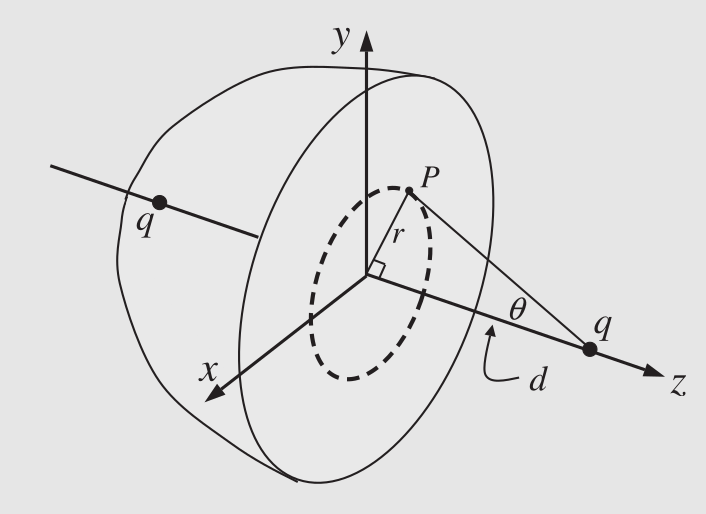
\includegraphics[width=0.35\linewidth]{3p18.png}

\end{figure}

\end{frame}

%-------------------------------------------------
\begin{frame}{Escolha da superfície}

\begin{mybox}
Escolhemos uma superfície $S$ em forma de “tigela”
\end{mybox}

\begin{itemize}
\item Ela envolve apenas a carga em $z=-d$
\item No limite:
\[
R \to \infty
\]
\item A parte hemisférica não contribui
\end{itemize}

\begin{alertblock}{Resultado chave}
A integral se reduz ao plano bissetor:
\[
z=0
\]
\end{alertblock}

\end{frame}

%-------------------------------------------------
\begin{frame}{Campo no plano bissetor}

\begin{mybox}
Por simetria:
\[
\hat n \cdot \mathbf E = 0
\]
\end{mybox}

\begin{itemize}
\item O campo está no plano
\item Apenas o termo $-\frac{1}{2}E^2 \hat n$ contribui
\end{itemize}

\begin{eqbox}
\begin{equation}
\mathbf F =
-\frac{\epsilon_0}{2}
\int_S dS\, E^2 \hat n
\end{equation}
\end{eqbox}

\end{frame}

%-------------------------------------------------
\begin{frame}{Geometria do problema}

\begin{mybox}
Definições:
\begin{itemize}
\item $\theta$: ângulo com o eixo $z$
\item distância até cada carga:
\[
r = \frac{d}{\cos\theta}
\]
\end{itemize}
\end{mybox}

\begin{itemize}
\item Usamos coordenadas cilíndricas no plano $z=0$
\end{itemize}

\end{frame}

%-------------------------------------------------
\begin{frame}{Campo elétrico no plano}

Campo de uma carga:

\begin{eqbox}
\begin{equation}
E = \frac{q}{4\pi\epsilon_0 r^2}
\end{equation}
\end{eqbox}

Com duas cargas:

\begin{eqbox}
\begin{equation}
E_{\parallel} = 2 \frac{q}{4\pi\epsilon_0 r^2}\cos\theta \sin\theta
\end{equation}
\end{eqbox}

Substituindo $r$:

\begin{eqbox}
\begin{equation}
E_{\parallel}
= 2 \frac{q}{4\pi\epsilon_0 d^2}
\cos^2\theta \sin\theta
\end{equation}
\end{eqbox}

\end{frame}

%-------------------------------------------------
\begin{frame}{Elemento de área}

No plano:

\begin{eqbox}
\begin{equation}
dS = r\,dr\,d\phi
\end{equation}
\end{eqbox}

Como:

\[
r = d \tan\theta
\]

\[
dr = d \frac{1}{\cos^2\theta} d\theta
\]

Logo:

\begin{eqbox}
\begin{equation}
dS = d^2 \frac{\sin\theta}{\cos^3\theta} d\theta d\phi
\end{equation}
\end{eqbox}

\end{frame}

%-------------------------------------------------
\begin{frame}{Montando a integral}

\begin{eqbox}
\begin{equation}
\mathbf F =
-\frac{\epsilon_0}{2}
\int dS\, E^2 \hat z
\end{equation}
\end{eqbox}

Substituindo $E$:

\begin{eqbox}
\begin{equation}
E^2 =
\left[
2 \frac{q}{4\pi\epsilon_0 d^2}
\cos^2\theta \sin\theta
\right]^2
\end{equation}
\end{eqbox}

\end{frame}

%-------------------------------------------------
\begin{frame}{Integral completa}

\begin{eqbox}
\begin{equation}
F_z =
-\frac{\epsilon_0}{2}
\left(
2 \frac{q}{4\pi\epsilon_0 d^2}
\right)^2
\int_0^{2\pi} d\phi
\int_0^{\pi/2}
\cos^4\theta \sin^2\theta
\cdot
\frac{\sin\theta}{\cos^3\theta}
d\theta
\end{equation}
\end{eqbox}

Simplificando:

\[
\cos^4\theta / \cos^3\theta = \cos\theta
\]

\[
\sin^2\theta \cdot \sin\theta = \sin^3\theta
\]

\end{frame}

%-------------------------------------------------
\begin{frame}{Integral simplificada}

\begin{eqbox}
\begin{equation}
F_z =
-\frac{\epsilon_0}{2}
\left(
2 \frac{q}{4\pi\epsilon_0 d^2}
\right)^2
\int_0^{2\pi} d\phi
\int_0^{\pi/2}
\cos\theta \sin^3\theta d\theta
\end{equation}
\end{eqbox}

Separando:

\[
\int_0^{2\pi} d\phi = 2\pi
\]

\end{frame}

%-------------------------------------------------
\begin{frame}{Integral angular}

\begin{eqbox}
\begin{equation}
I = \int_0^{\pi/2} \cos\theta \sin^3\theta d\theta
\end{equation}
\end{eqbox}

Substituição:

\[
u = \sin\theta \Rightarrow du = \cos\theta d\theta
\]

\begin{eqbox}
\begin{equation}
I = \int_0^1 u^3 du = \frac{1}{4}
\end{equation}
\end{eqbox}

\end{frame}

%-------------------------------------------------
\begin{frame}{Resultado final}

\begin{eqbox}
\begin{equation}
F =
-\hat z
\frac{q^2}{4\pi\epsilon_0 (2d)^2}
\end{equation}
\end{eqbox}

\begin{mybox}
Resultado:
\begin{itemize}
\item Lei de Coulomb recuperada
\item Direção correta (repulsão)
\end{itemize}
\end{mybox}

\end{frame}

%-------------------------------------------------
\begin{frame}{Interpretação física}

\begin{mybox}
O que aprendemos:
\end{mybox}

\begin{itemize}
\item A força surge do campo no espaço vazio
\item O campo exerce uma pressão
\item A interação é mediada pelo tensor de tensões
\end{itemize}

\begin{alertblock}{Mensagem central}
Campos carregam momento e transmitem forças
\end{alertblock}

\end{frame}


\end{document}